\documentclass[aspectratio=149, xcolor=table]{beamer}
%\usetheme{Montpellier}
%\usecolortheme{dove}
%\useinnertheme{rounded}
%\useoutertheme{smoothbars}
\usetheme{Madrid}
\usefonttheme{serif}
\usecolortheme{dove}
\useinnertheme{rounded}
\useoutertheme{miniframes}
\usepackage{booktabs}
\setbeamersize{text margin left=5mm,text margin right=10mm}
\usepackage{graphicx}
\usepackage{multicol}
\usepackage{animate}
\usepackage{appendixnumberbeamer}
\setbeamertemplate{navigation symbols}[horizontal] 
\setbeamersize{text margin left=5mm,text margin right=5mm} 
\setbeamercolor{subsection name}{fg=white}
\setbeamercolor{section name}{fg=white}
%\setbeamercolor{title}{bg=white, fg=rasch}
%\setbeamercolor{frame title}{bg=white, fg=rasch}
%\setbeamerfont{frame title}{family=\bfseries}
\setbeamerfont{section title}{family=\bfseries}
\setbeamerfont{title}{family=\bfseries}
\usepackage{xcolor}
\usepackage{tikz}
\usepackage[absolute,overlay]{textpos}
\usepackage{spot}
\usepackage{tikzsymbols}
%\usepackage[raggedright]{titlesec}
\usetikzlibrary{mindmap,calc,patterns,decorations.pathmorphing,decorations.markings, arrows, shapes.arrows, shapes, backgrounds}
\definecolor{unipd}{RGB}{155, 0, 20}
\definecolor{grigioPantano}{RGB}{72,79,89}
\definecolor{template}{RGB}{72,79,89}
\definecolor{royalblue3}{RGB}{58,95,205}

\usetikzlibrary{shapes.geometric, arrows}
\tikzstyle{respondent} = [rectangle, minimum width=1.5cm, minimum height=1cm,text centered, draw=white]
\tikzstyle{stimulus} = [rectangle, minimum width=1.5cm, minimum height=1cm,text centered, draw=white]
\tikzstyle{trial} = [rectangle, minimum width=1cm, minimum height=1cm,text centered, draw=black]
\tikzstyle{process} = [rectangle, rounded corners, minimum width=0.5cm, minimum height=1cm, text width =2.5cm, text centered, draw=black]
\tikzstyle{arrow} = [thick,->,>=stealth]
\tikzstyle{condition} = [rectangle, rounded corners,draw=black,text width=2cm, text height=6.5cm]
\tikzstyle{latent} = [ellipse, minimum width=2.5cm, minimum height=2cm,text centered, draw=black]
\tikzstyle{item} = [rectangle, rounded corners, minimum width=0.5cm, minimum height=1cm, text width =1.5cm, text centered, draw=black]
\tikzstyle{arrow} = [thick,->,>=stealth]
\setbeamerfont{block title}{family=\bfseries}
\setbeamercolor{block title}{use=structure,fg=unipd,bg=white}
%\setbeamercolor{block body}{fg=black,use=block title,bg=grigioPantano!10}
%
%
%\setbeamercolor{block title example}{use=example text,fg=white,bg=green!50!black}
%\setbeamercolor{block body example}{fg=grigioPantano!60!black,use=block title example,bg=grigioPantano!10}
%
%\setbeamercolor{block title alerted}{use=alerted text,fg=white,bg=unipd}
%\setbeamercolor{block body alerted}{fg=black,use=block title alerted,bg=grigioPantano!20}


  \tikzset{
	invisible/.style={opacity=0},
	visible on/.style={alt={#1{}{invisible}}},
	alt/.code args={<#1>#2#3}{%
		\alt<#1>{\pgfkeysalso{#2}}{\pgfkeysalso{#3}} % \pgfkeysalso doesn't change the path
	},
	every overlay node/.style={
		%draw=black,fill=white,rounded corners,
		anchor=north west, inner sep=0pt,
	},
}

% \title[Randomness and possibilities]{When randomness opens new possibilities: Acknowledging the stimulus sampling variability in Experimental Psychology}
%\vspace{-1.5mm}\author[OME, PA, ER]{ Ottavia M. Epifania\textsuperscript{1,2,3}, Pasquale Anselmi\textsuperscript{1}, Egidio Robusto\textsuperscript{1}\\ \texttt{ottavia.epifania@unipd.it}}
%\institute[]{\small \textsuperscript{1} University of Padova (IT) \\
%\textsuperscript{2} Psicostat Group \\
%\textsuperscript{3} Catholic Univerisity of the Sacred Heart, Milan (IT) \\}
%\vspace*{-5mm}
%\date[CMS Conference]{\footnotesize Conference CMS Berlin \\ December 16}
%\titlegraphic{\vspace{-5mm}%
%	
\includegraphics[width=1.5cm,height=1.5cm,keepaspectratio]{img/unipd.png}%\hspace*{9.75cm}~%
%	
\includegraphics[width=2cm,height=2cm,keepaspectratio]{img/psicostat.png}%
%	
\includegraphics[width=1.5cm,height=1.5cm,keepaspectratio]{img/unicatt.png}%
%}

\definecolor{back}{RGB}{247, 251, 255}
\definecolor{map}{RGB}{111, 172, 232}
\definecolor{childmap}{RGB}{161, 200, 240}
\definecolor{nodemap}{RGB}{141, 170, 199}
\definecolor{rasch}{rgb}{0.0, 0.33, 0.71}
\definecolor{log}{rgb}{0.0, 0.65, 0.58}
\definecolor{diff}{RGB}{33, 113, 181}
\definecolor{single}{RGB}{106, 81, 163}
\definecolor{comp}{RGB}{35, 99, 70}
\definecolor{inc}{RGB}{191, 13, 43}
\definecolor{highlight}{rgb}{0.45, 0.31, 0.59}
\definecolor{section}{RGB}{51,51,179}
\definecolor{typical}{RGB}{8, 69, 148}
\definecolor{model}{RGB}{74, 20, 134}
\definecolor{orangered2}{RGB}{238,64,0}
\definecolor{royalblue3}{RGB}{58,95,205}
\definecolor{springgreen}{RGB}{0,205,102}
\definecolor{magenta}{RGB}{255,0,255}
\def\tikzoverlay{%
	\tikz[remember picture, overlay]\node[every overlay node]
}%

%\AtBeginSubsection{\frame{\subsectionpage}}
 \AtBeginSection{\frame{\sectionpage}}
\setbeamertemplate{subsection page}
{
	\begingroup
	\begin{beamercolorbox}[sep=12pt,center]{section title}
		\usebeamerfont{section title}\insertsection\par
	\end{beamercolorbox}
	\vspace*{5pt}
	\begin{beamercolorbox}[sep=8pt,center]{subsection title}
		\usebeamerfont{subsection title}\insertsubsection\par
	\end{beamercolorbox}
	\endgroup
}
\title[Research activity]{Research activity, interests and beyond}
%\subtitle{Voglio morire}
\vspace{-2.5mm}
\author[Epifania O.M.]{Ottavia M. Epifania, Ph.D.}


\date [May 22\textsuperscript{nd}] {%\vspace{0.6cm}\\
	\small
	Università di Trento\\ Rovereto, Italia \\ \vspace{3mm}
	May, 22\textsuperscript{nd} 2024}

\institute [] {
	%
\includegraphics[width=1.5cm,height=1.5cm,keepaspectratio]{img/unipd.png}%\hspace*{9.75cm}~%
	\centering

\includegraphics[width=3.5cm,height=3.5cm,keepaspectratio]{img/psicostat.png}%
%
\includegraphics[width=1.5cm,height=1.5cm,keepaspectratio]{img/unicatt.png}\\ 
}

\begin{document}
\begin{frame}[plain]
    \maketitle
    \end{frame}


\begin{frame}{Item Response Theory and Rasch modeling}


\begin{footnotesize}
			\begin{verbatim}
		
		( TITLE-ABS-KEY ( "Item response theory" )  OR  TITLE-ABS-KEY ( "Rasch" ) )  
		
		AND PUBYEAR > 1959  AND  PUBYEAR  <  2025  
		AND  ( LIMIT-TO ( DOCTYPE ,  "ar" ) ) 
	\end{verbatim}
	
\end{footnotesize}

$n = 18,661$ documents (May, 17\textsuperscript{th} 2024) on Scopus: 

\begin{columns}[T]
	\begin{column}{.50\linewidth}
		\centering
		Some fields of application: 
	\begin{figure}
		\centering
		
\includegraphics[width=.7\linewidth]{img/wordcloud.png}
	\end{figure}
	\end{column}
		\begin{column}{.50\linewidth}
			\begin{center}
			Some reasons for their application: 
			\end{center}
			
	Measure validation \\\vspace{1.5mm} Measure refinement \\ \vspace{1.5mm}Item selection \\\vspace{1.5mm} Computerized Adaptive testing \\\vspace{1.5mm} $\ldots$
	\end{column}
\end{columns}



\end{frame}


\begin{frame}
	\centering
	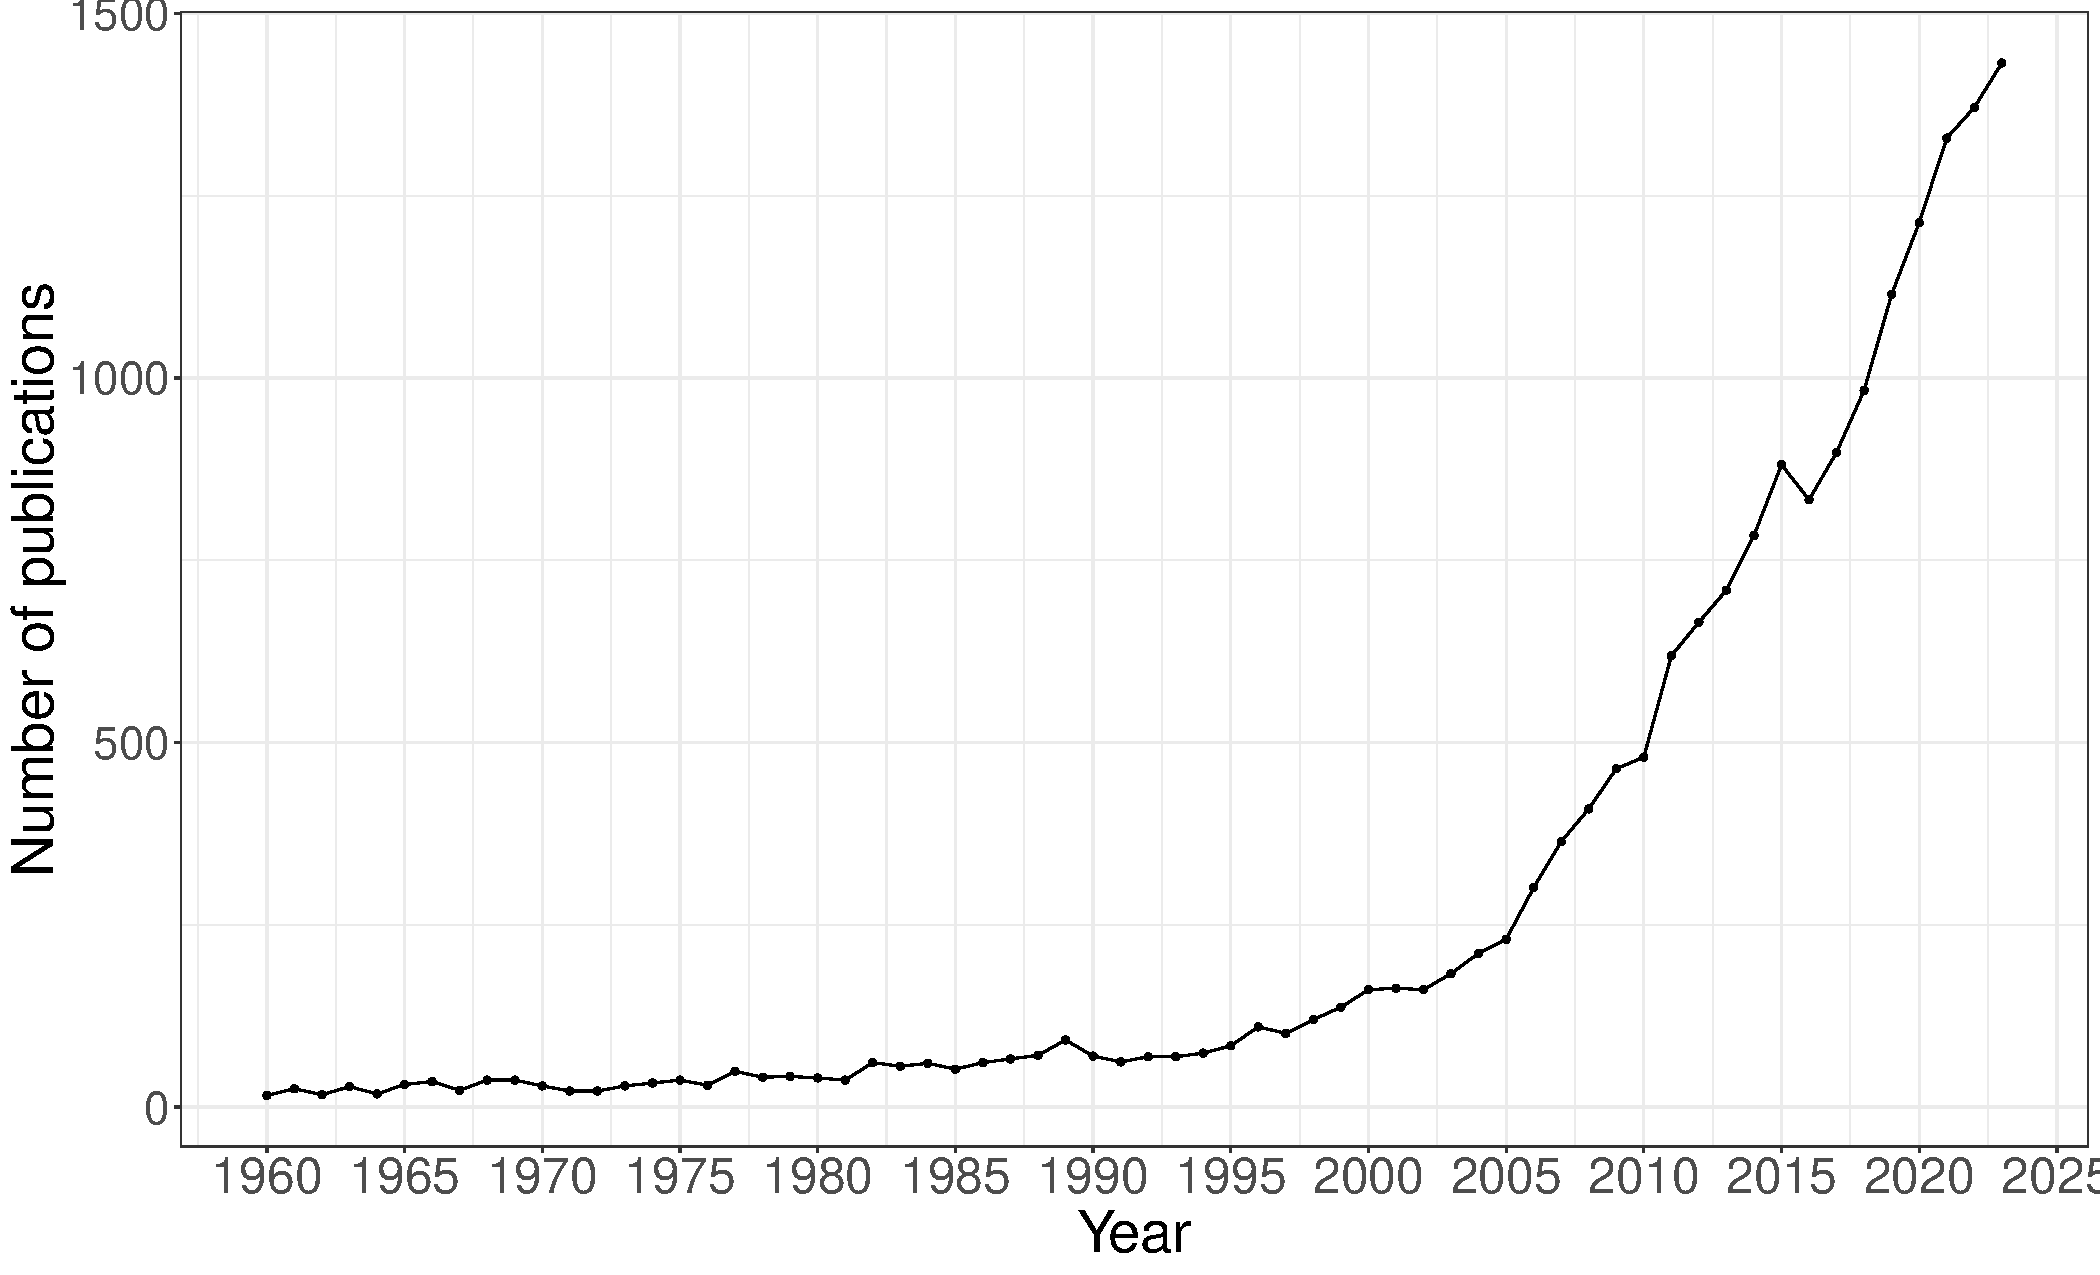
\includegraphics[width=.80\linewidth]{freq-year.pdf}
%		\centering
%	\animategraphics[autoplay,width=0.80\linewidth]{15}{animate/gganim_plot}{0001}{0100}
\end{frame}

\begin{frame}{My research activity and interests}
	\tableofcontents
\end{frame}

\section[Rasch revised \& beyond]{Rasch modeling of complex data structures}

\begin{frame}
	\onslide<1->
	\tikzoverlay (bart) at (-0.5cm,2.2cm) {%
		\begin{minipage}{.20\textwidth}
			\begin{figure}
				\centering
				
\includegraphics[width=.90\linewidth]{img/bart.png}
			\end{figure}
		\end{minipage}
	};
	\tikzoverlay (bart1) at (-0.5cm,-1.3cm) {%
		\begin{minipage}{.20\textwidth}
			\centering
			$A_\text{Bart}$
			
		\end{minipage}
	};
	\tikzoverlay (lisa) at (9.5cm,1.5cm) {%
		\begin{minipage}{.20\textwidth}
			\begin{figure}
				\centering
				
\includegraphics[width=.80\linewidth]{img/lisa.png}
			\end{figure}
		\end{minipage}
	};
	
	\tikzoverlay (lisa1) at (9.9cm,-0.8cm) {%
		\begin{minipage}{.20\textwidth}
			\centering
			$A_\text{Lisa}$
			
		\end{minipage}
	};
	\onslide<2->
	\tikzoverlay (math) at (2cm,2.0cm) {%
		\begin{minipage}{.60\textwidth}
			\begin{columns}[T]
				\begin{column}{.50\linewidth}
					\centering \textbf{Q1}
					\begin{equation*}
						4 + 5 = ?
					\end{equation*}
				\end{column}
				
				\begin{column}{.50\linewidth}
					\centering \textbf{Q2}
					\begin{equation*}
						\dfrac{3}{2}x^2 + \dfrac{5}{4}x = ?
					\end{equation*}
				\end{column}
			\end{columns}
		\end{minipage}
	};
	\tikzoverlay (math1) at (2cm,0.5cm) {%
		\begin{minipage}{.60\textwidth}
			\begin{columns}[T]
				
				\begin{column}{.50\linewidth}
					\begin{equation*}
						d_{q1}
					\end{equation*}
				\end{column}
				\begin{column}{.50\linewidth}
					\begin{equation*}
						d_{q2}
					\end{equation*}
				\end{column}
			\end{columns}
		\end{minipage}
	};
	
	\onslide<3->
	\tikzoverlay (eq) at (0.3cm, -1.5cm){
		\begin{minipage}{.30\linewidth}
			\begin{equation*}
				\dfrac{A_p}{d_i}
			\end{equation*}
			\centering
			\vspace{3mm}
			$> 1$ if $A_p > d_i$
			
			$< 1$ if $A_p < d_i$
		\end{minipage}
	};
	\tikzoverlay (eq1) at (5.3cm, -1.5cm){
		\begin{minipage}{.50\linewidth}
			\begin{equation*}
				P(X_{pi} = 1) = \dfrac{\dfrac{A_p}{d_i}}{1 + \dfrac{A_p}{d_i}}
			\end{equation*}
		\end{minipage}
	};
\end{frame}

\begin{frame}
%	\begin{figure}
%		\centering
%		
\includegraphics[width=0.3\linewidth]{img/later}
%	\end{figure}
%	\begin{columns}[T]
%		\begin{column}{.5\linewidth}
%			\centering
%			$ln(A_p) = \theta_p$
%		\end{column}
%		\begin{column}{.5\linewidth}
%			\centering
%			$ln(d_i) = b_i$
%		\end{column}
%	\end{columns}

	\begin{equation*}
		P(X_{pi} = 1|\theta_p, b_i) = \dfrac{\exp(\theta_p - b_i)}{1 + \exp(\theta_p - b_i)}
	\end{equation*}
	
	
		\begin{overprint}
		\centering
		\onslide<2>
			\centering
		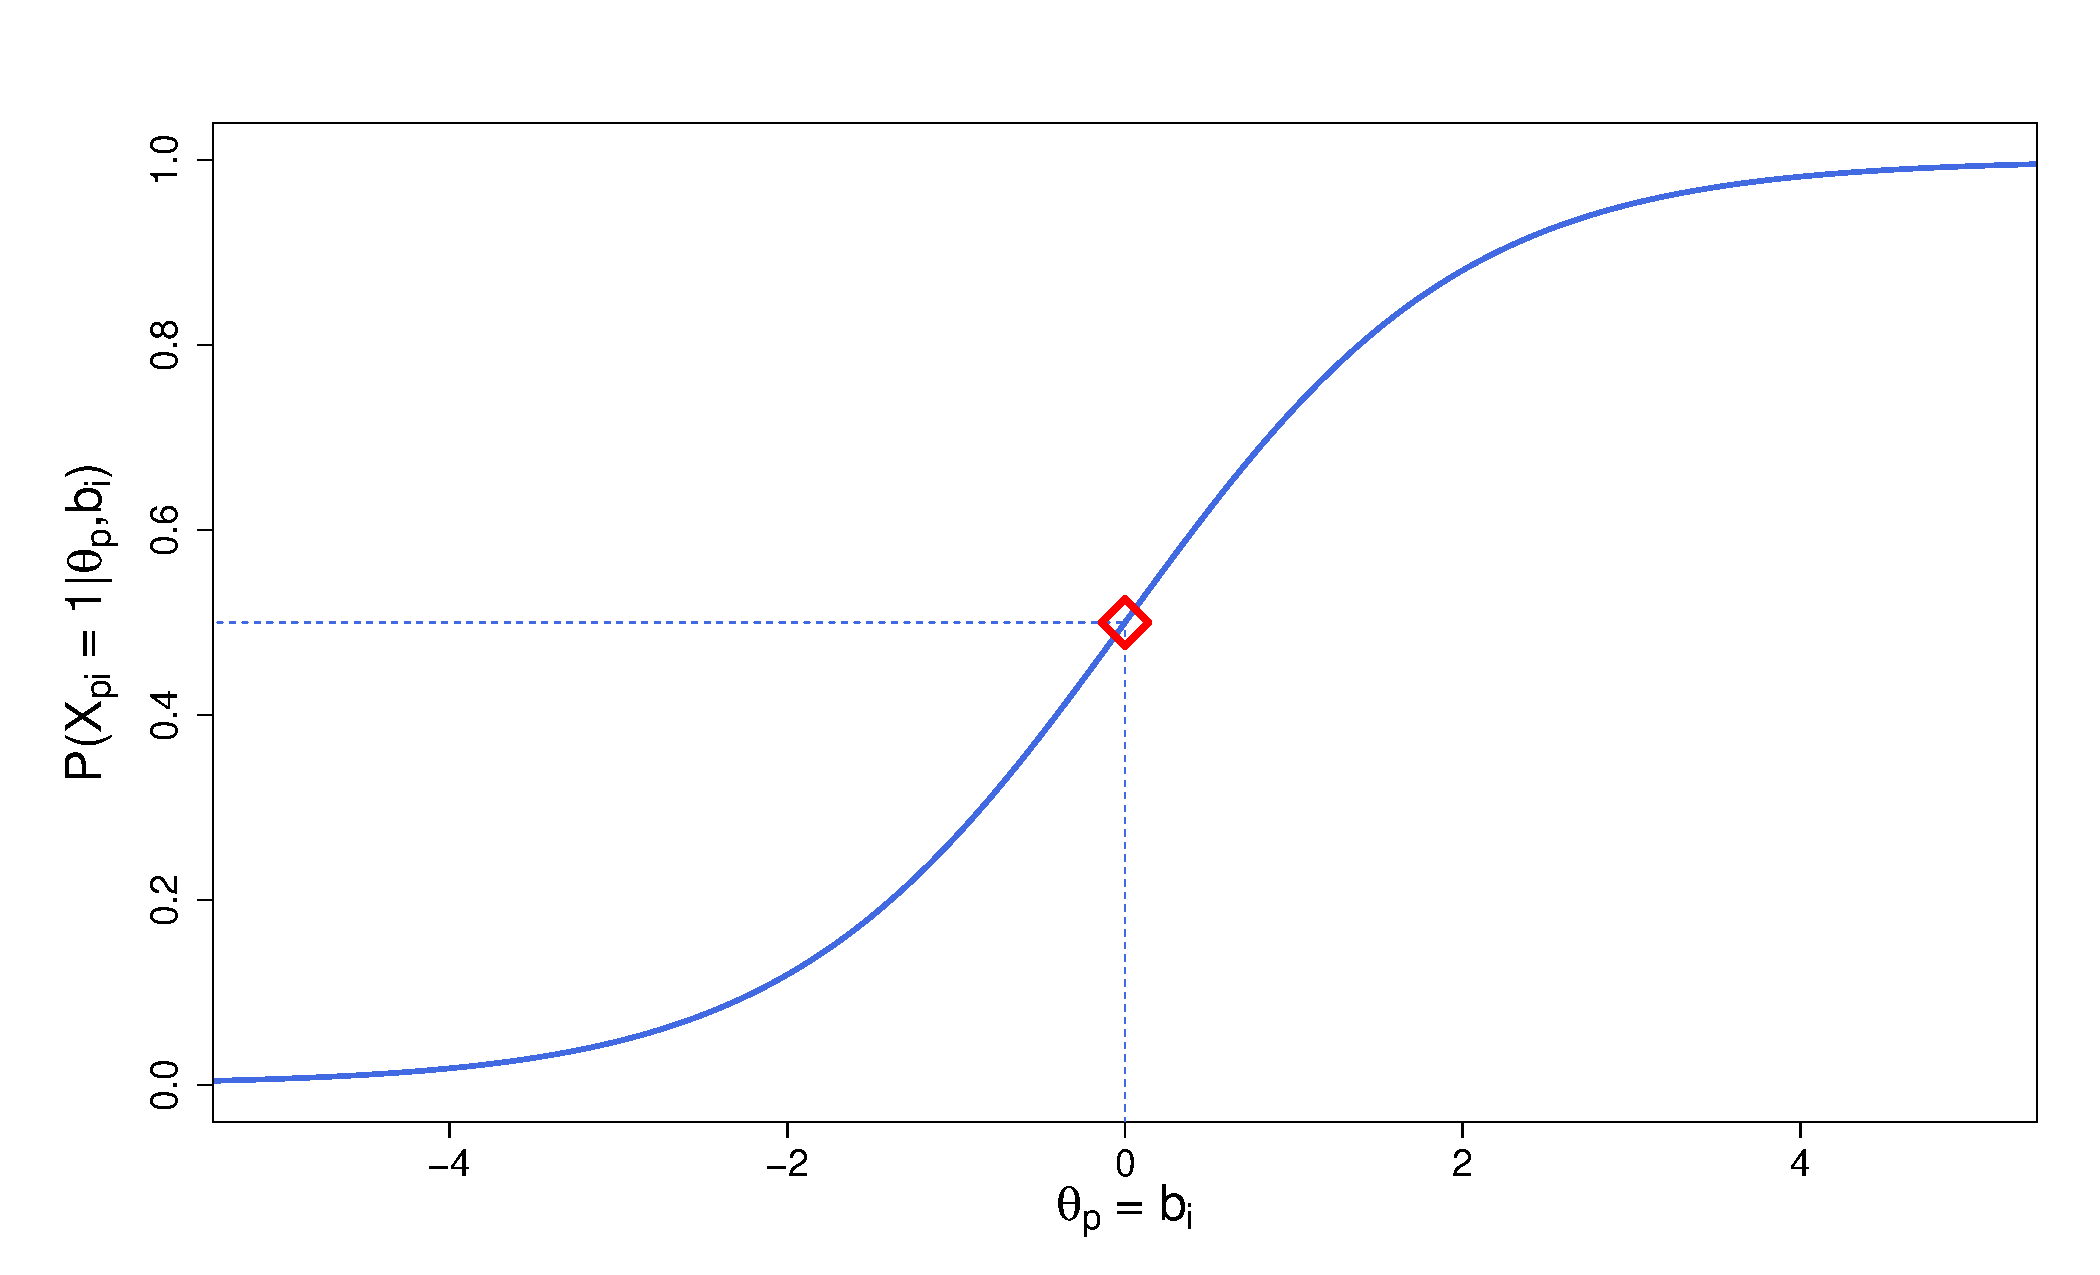
\includegraphics[width=.8\linewidth]{img/base.pdf}
		
		\centering
		\onslide<3>
			\centering
		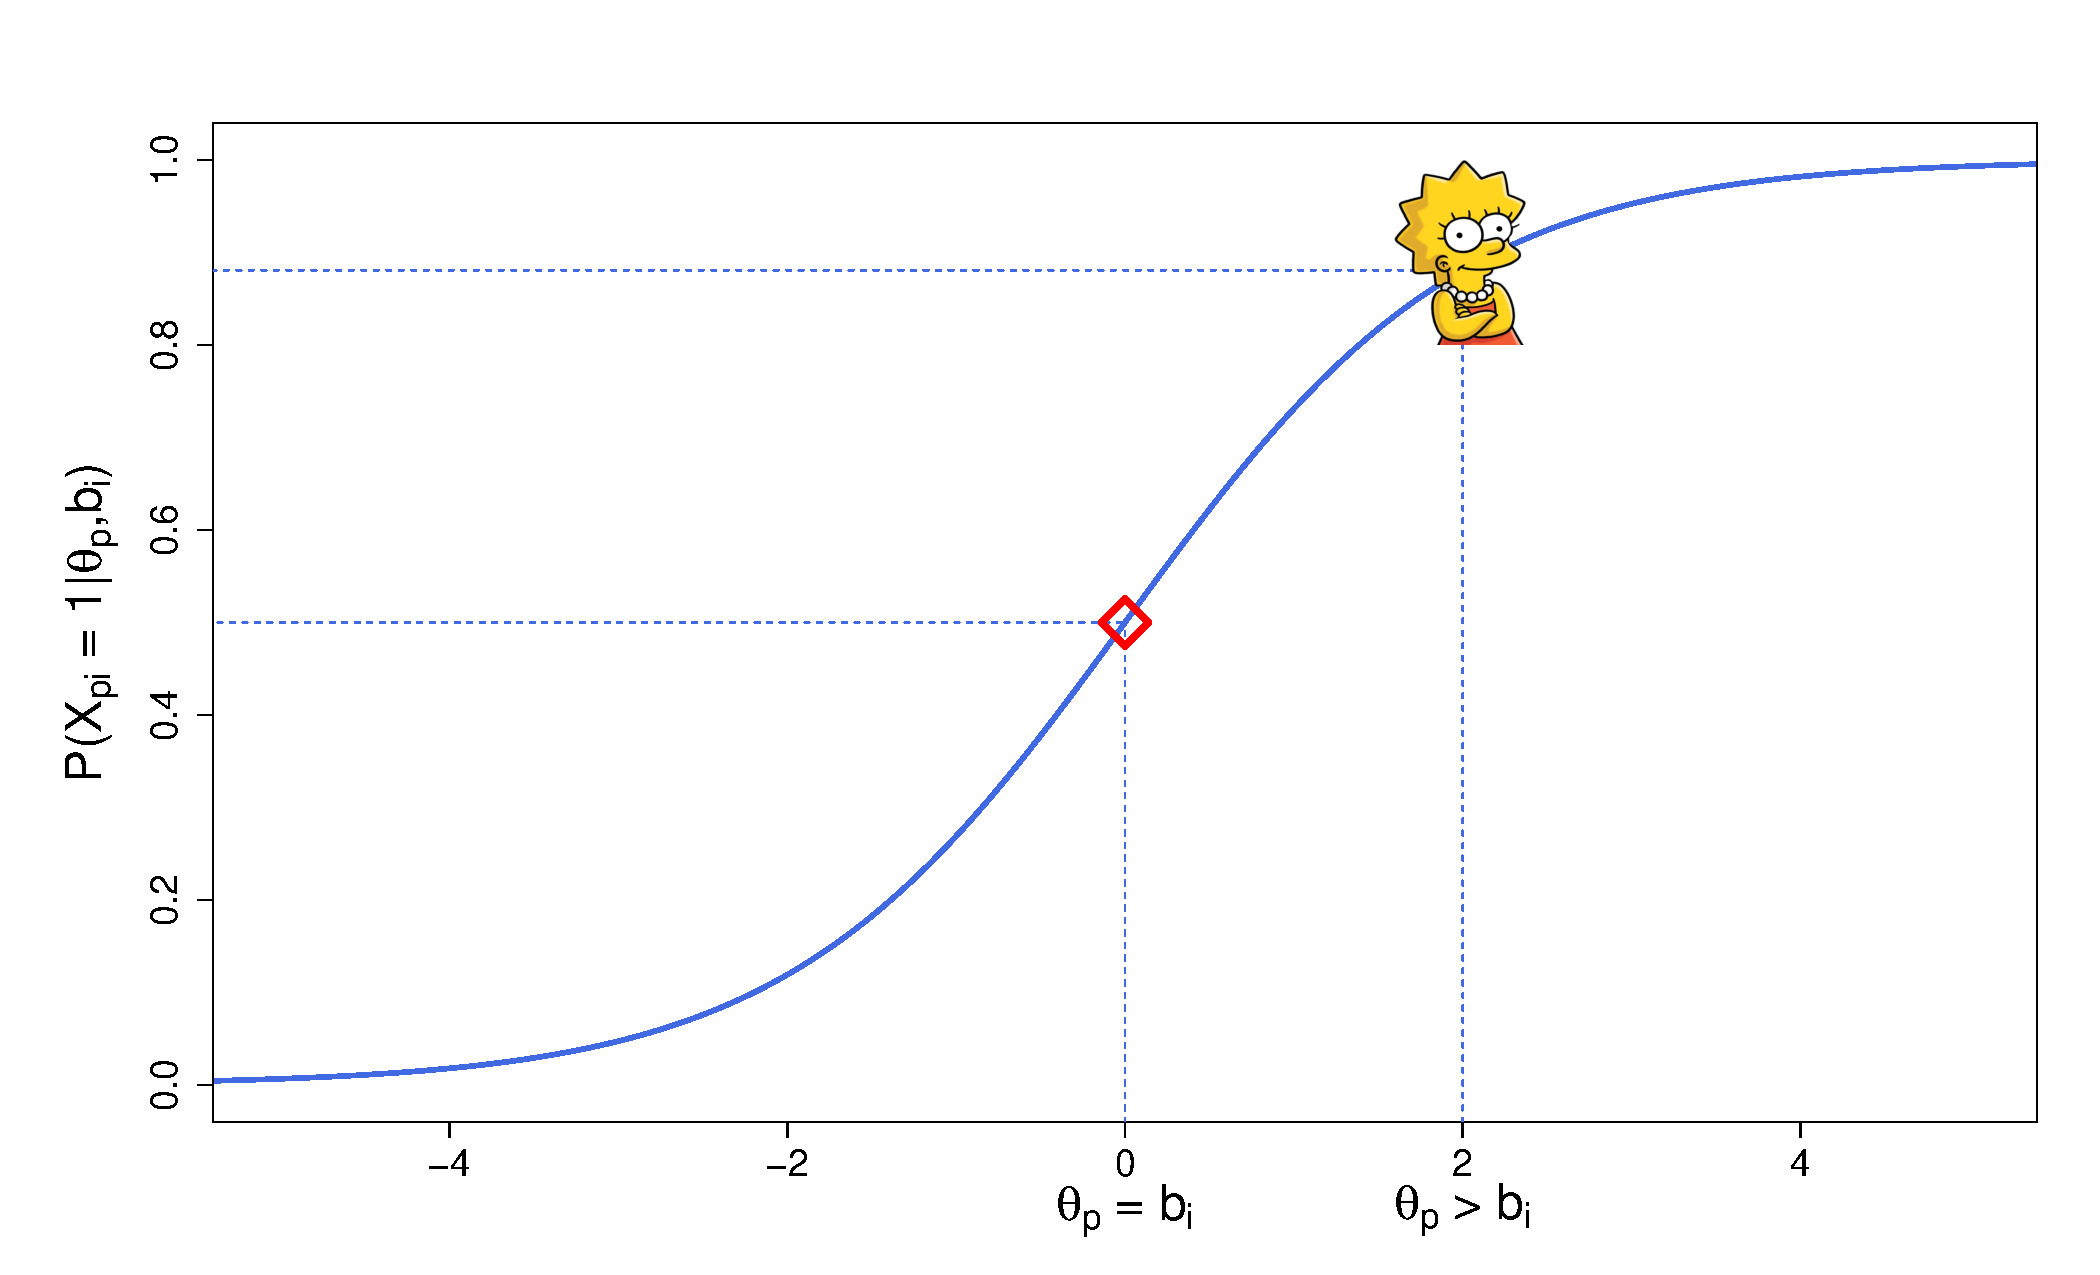
\includegraphics[width=.8\linewidth]{img/lisa.pdf}
		
		\centering
		\onslide<4>
			\centering
		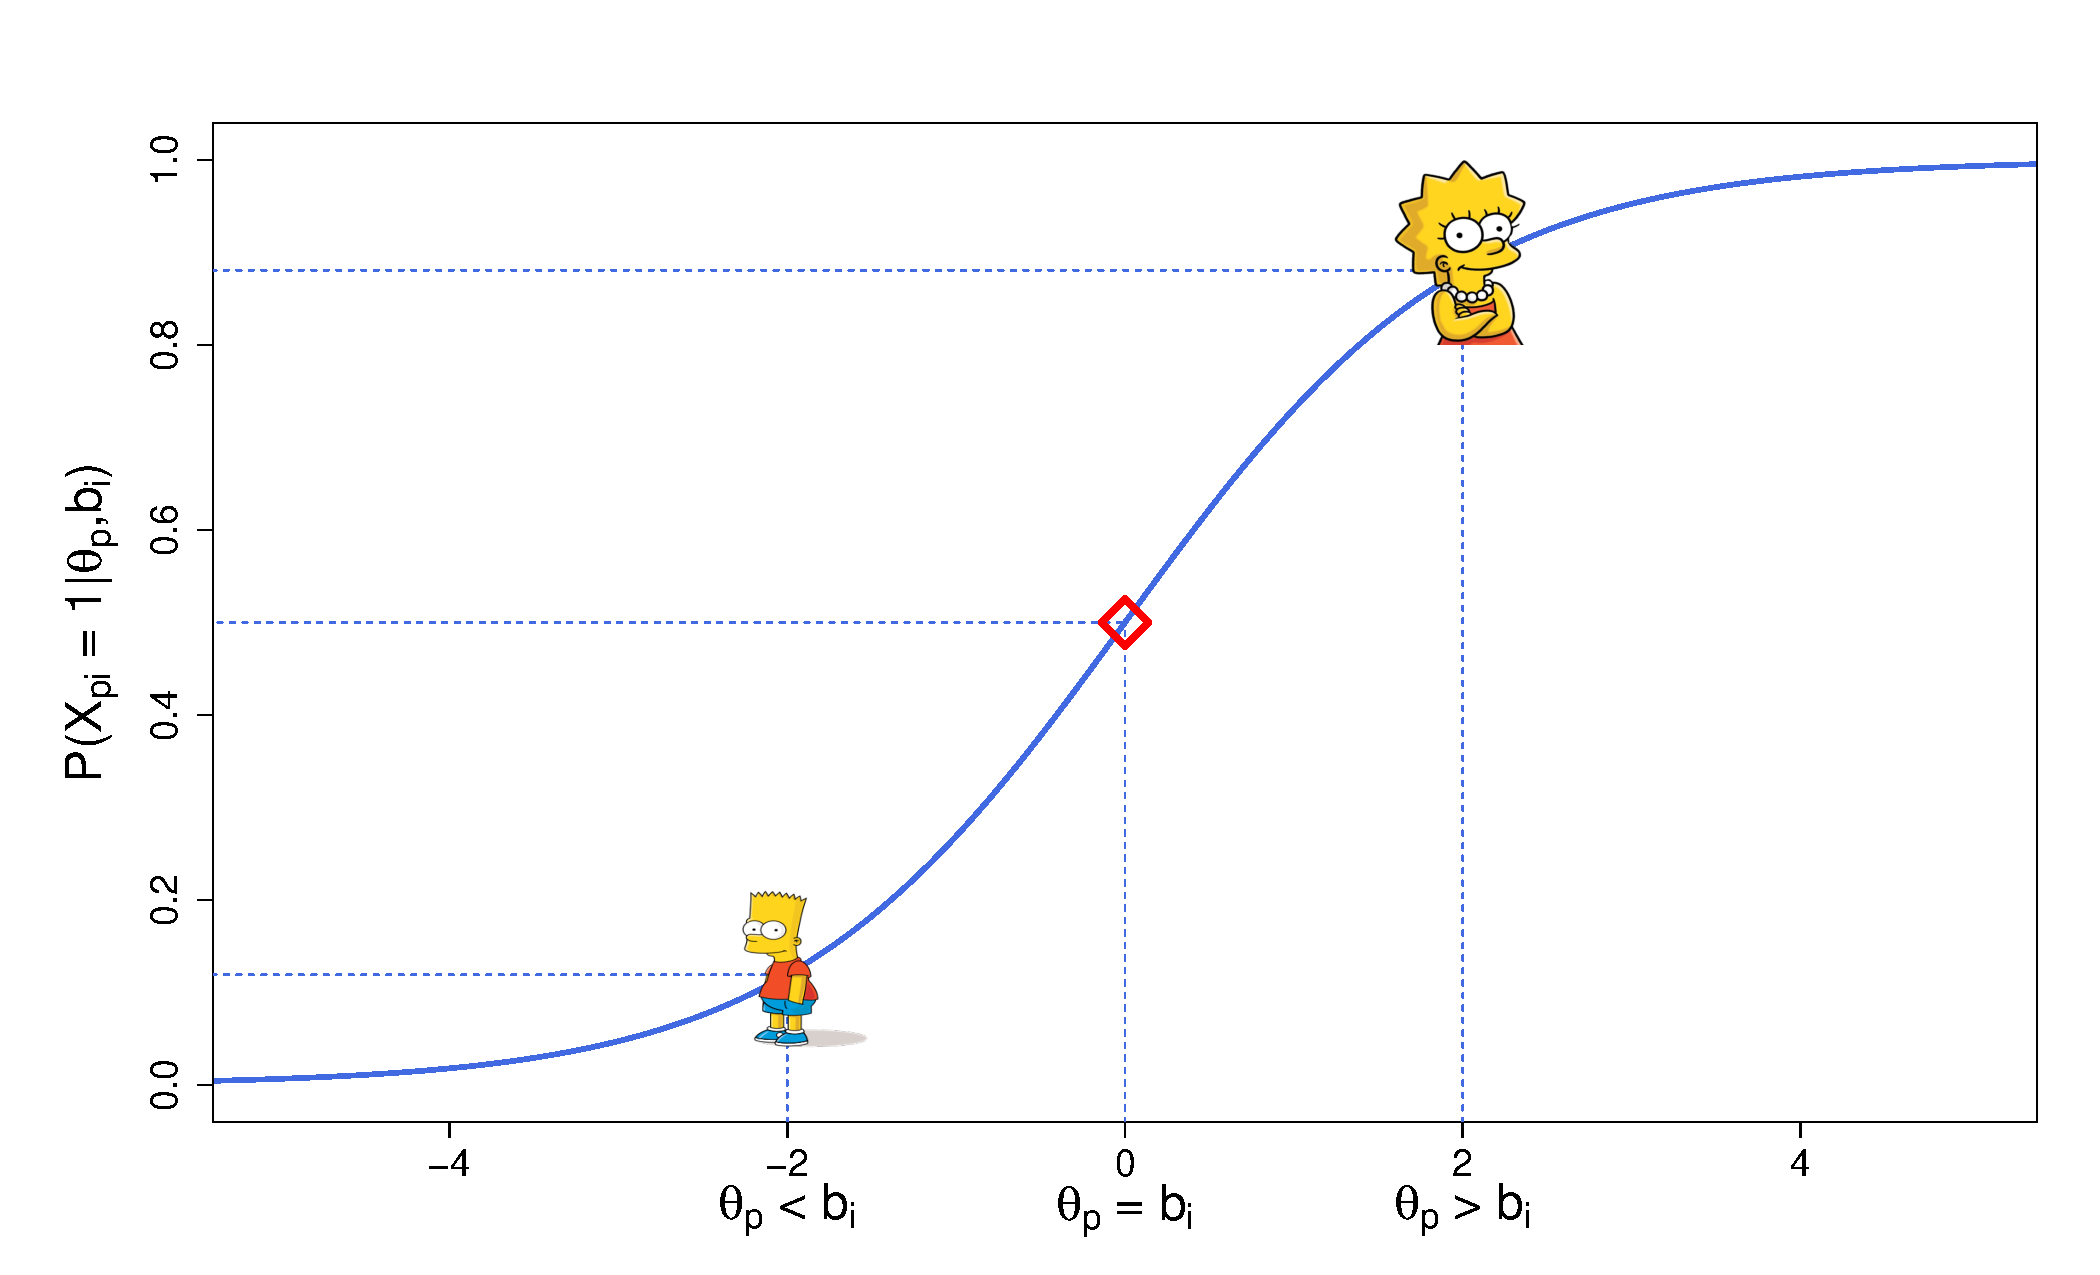
\includegraphics[width=.8\linewidth]{img/bart.pdf}
	\end{overprint}
	
\end{frame}

%\begin{frame}
%	\centering
%	
%	\begin{overprint}
%		
%		\onslide<1>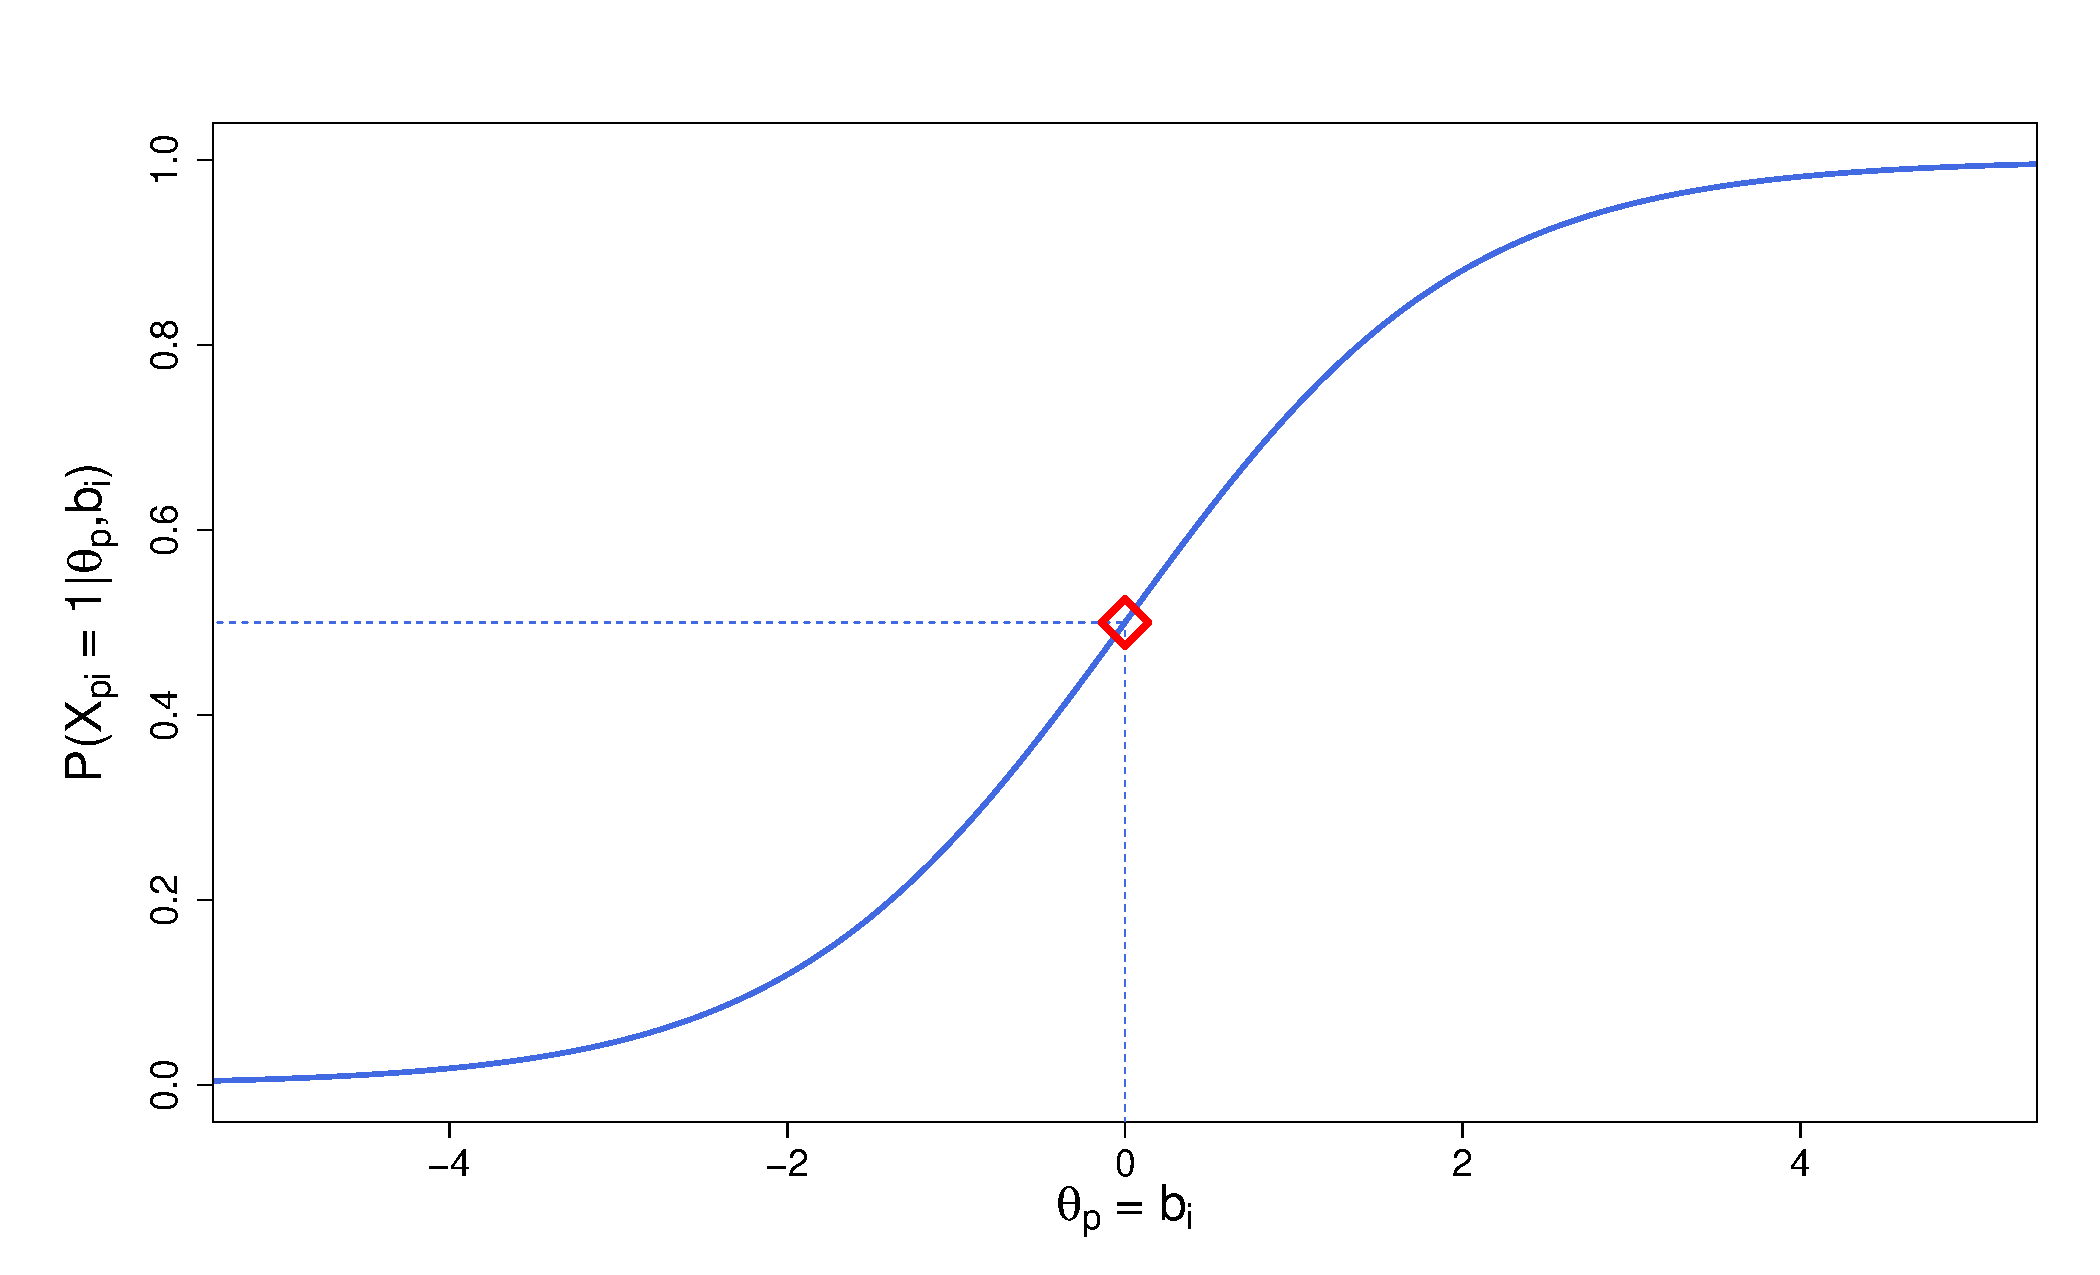
\includegraphics[width=\linewidth]{img/base.pdf}
%		\onslide<2>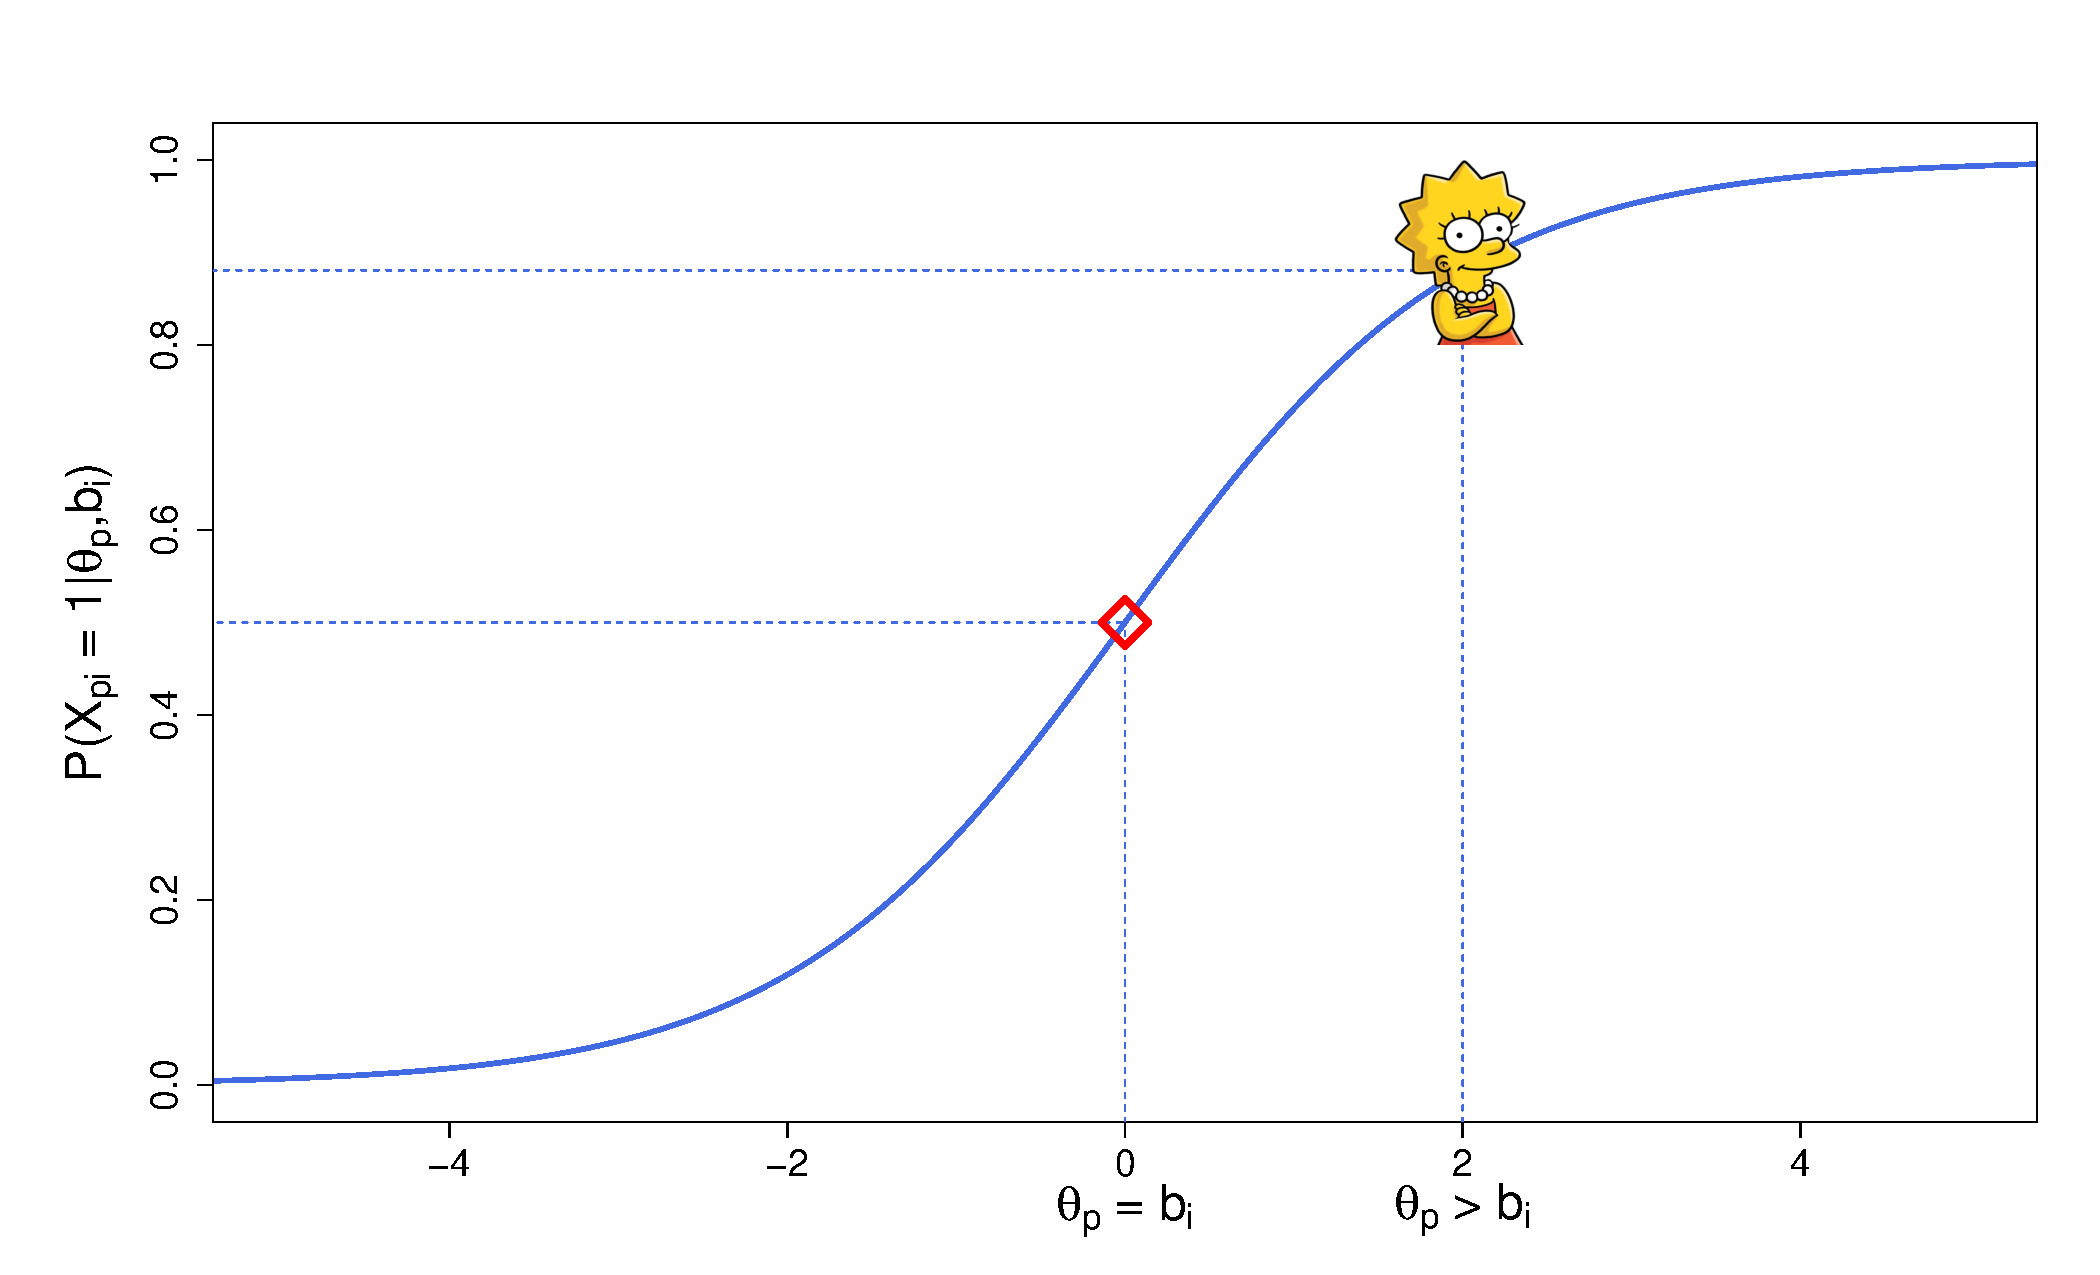
\includegraphics[width=\linewidth]{img/lisa.pdf}
%		\onslide<3>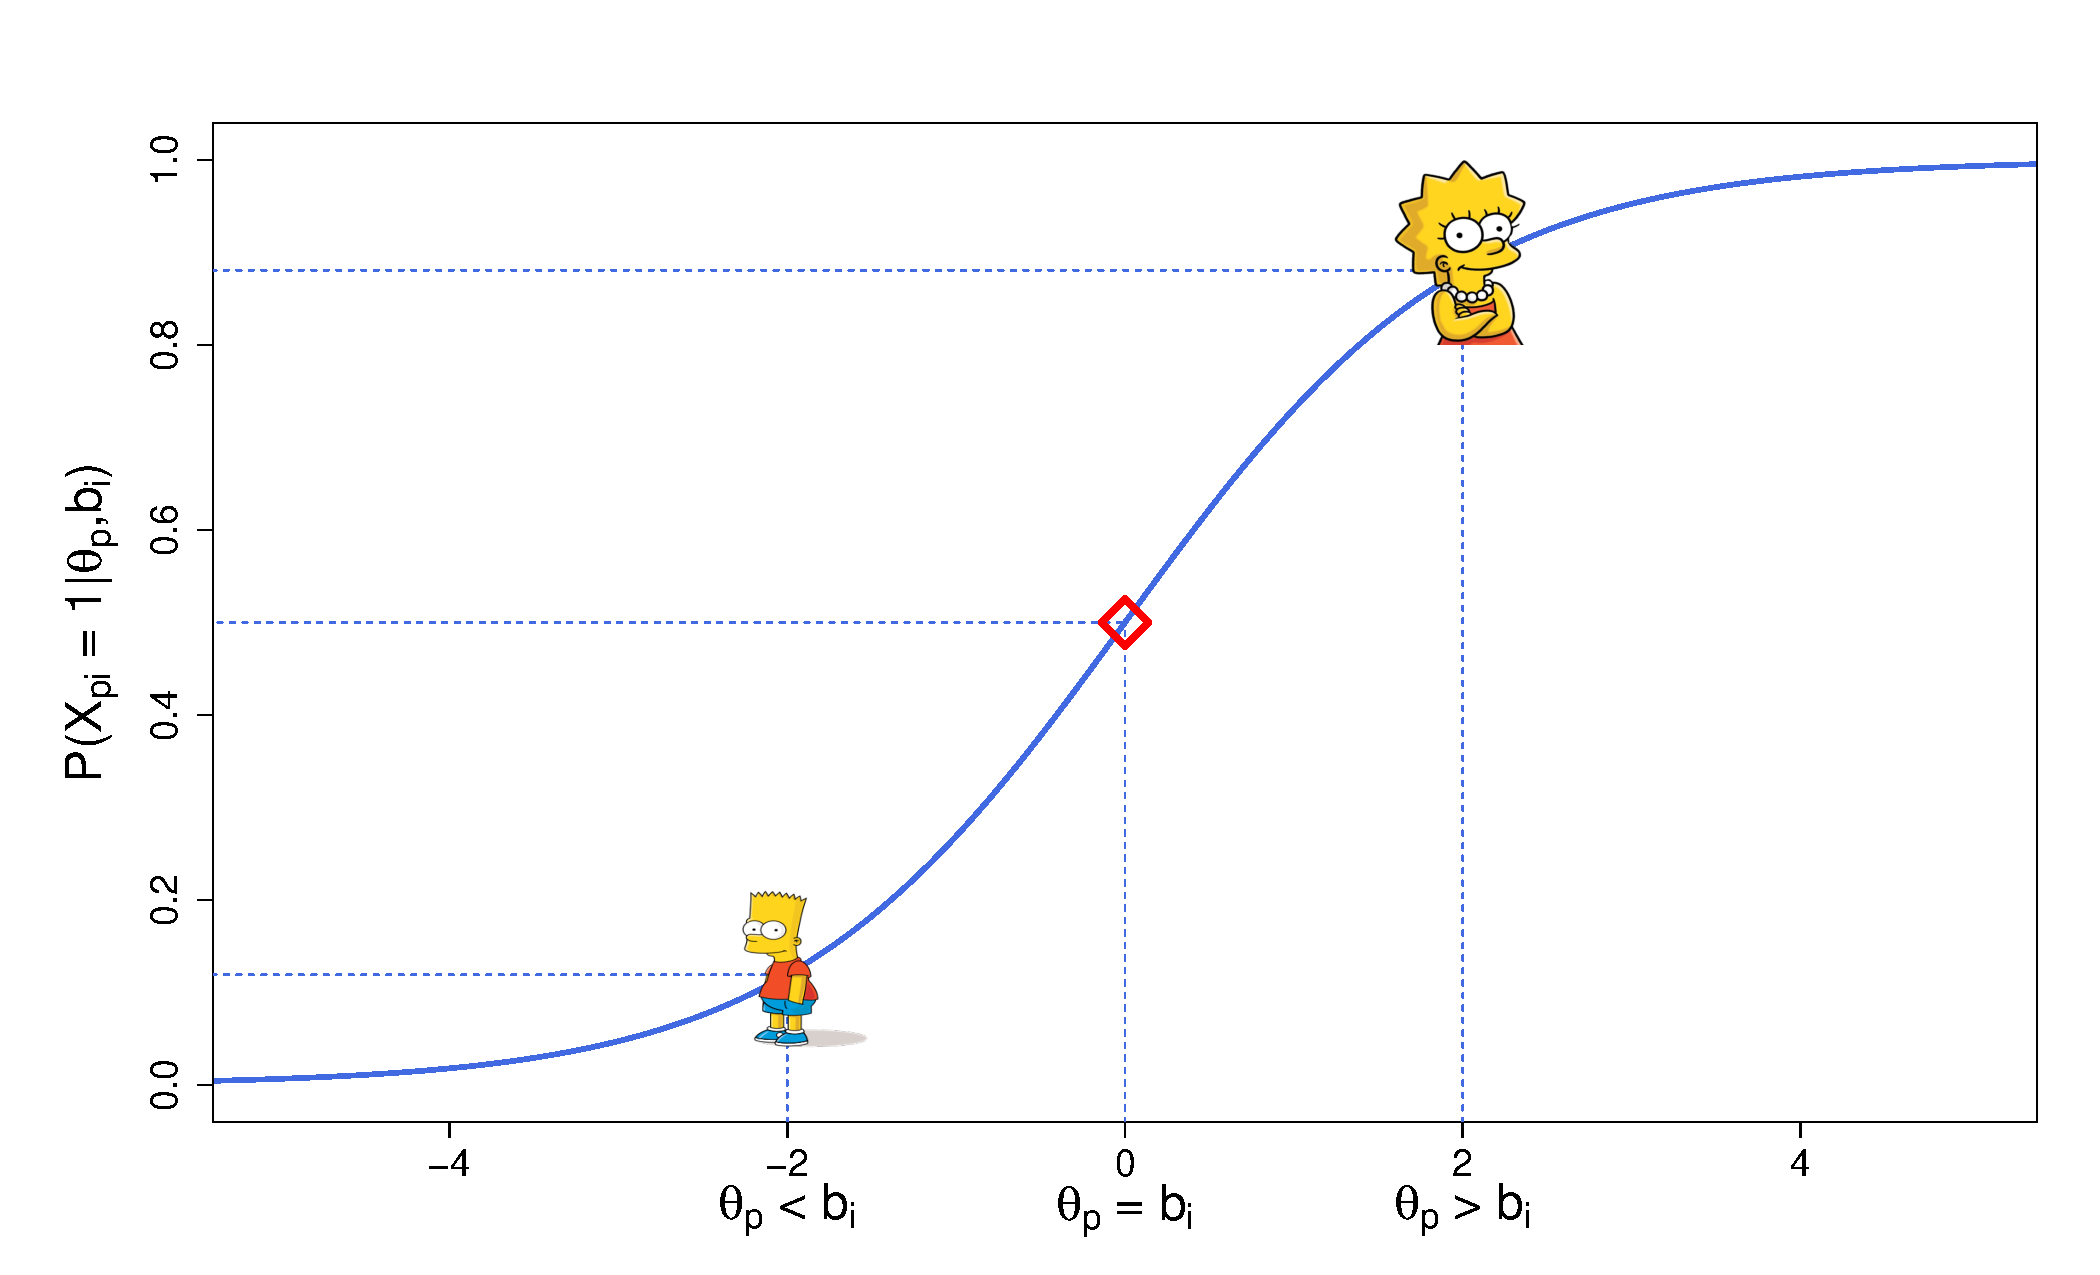
\includegraphics[width=\linewidth]{img/bart.pdf}
%		
%		
%	\end{overprint}
%	
%\end{frame}


\begin{frame}{Generalized linear model (GLM) for dichotomous responses}
	
	\begin{figure}
		\begin{overprint}
			\onslide<1>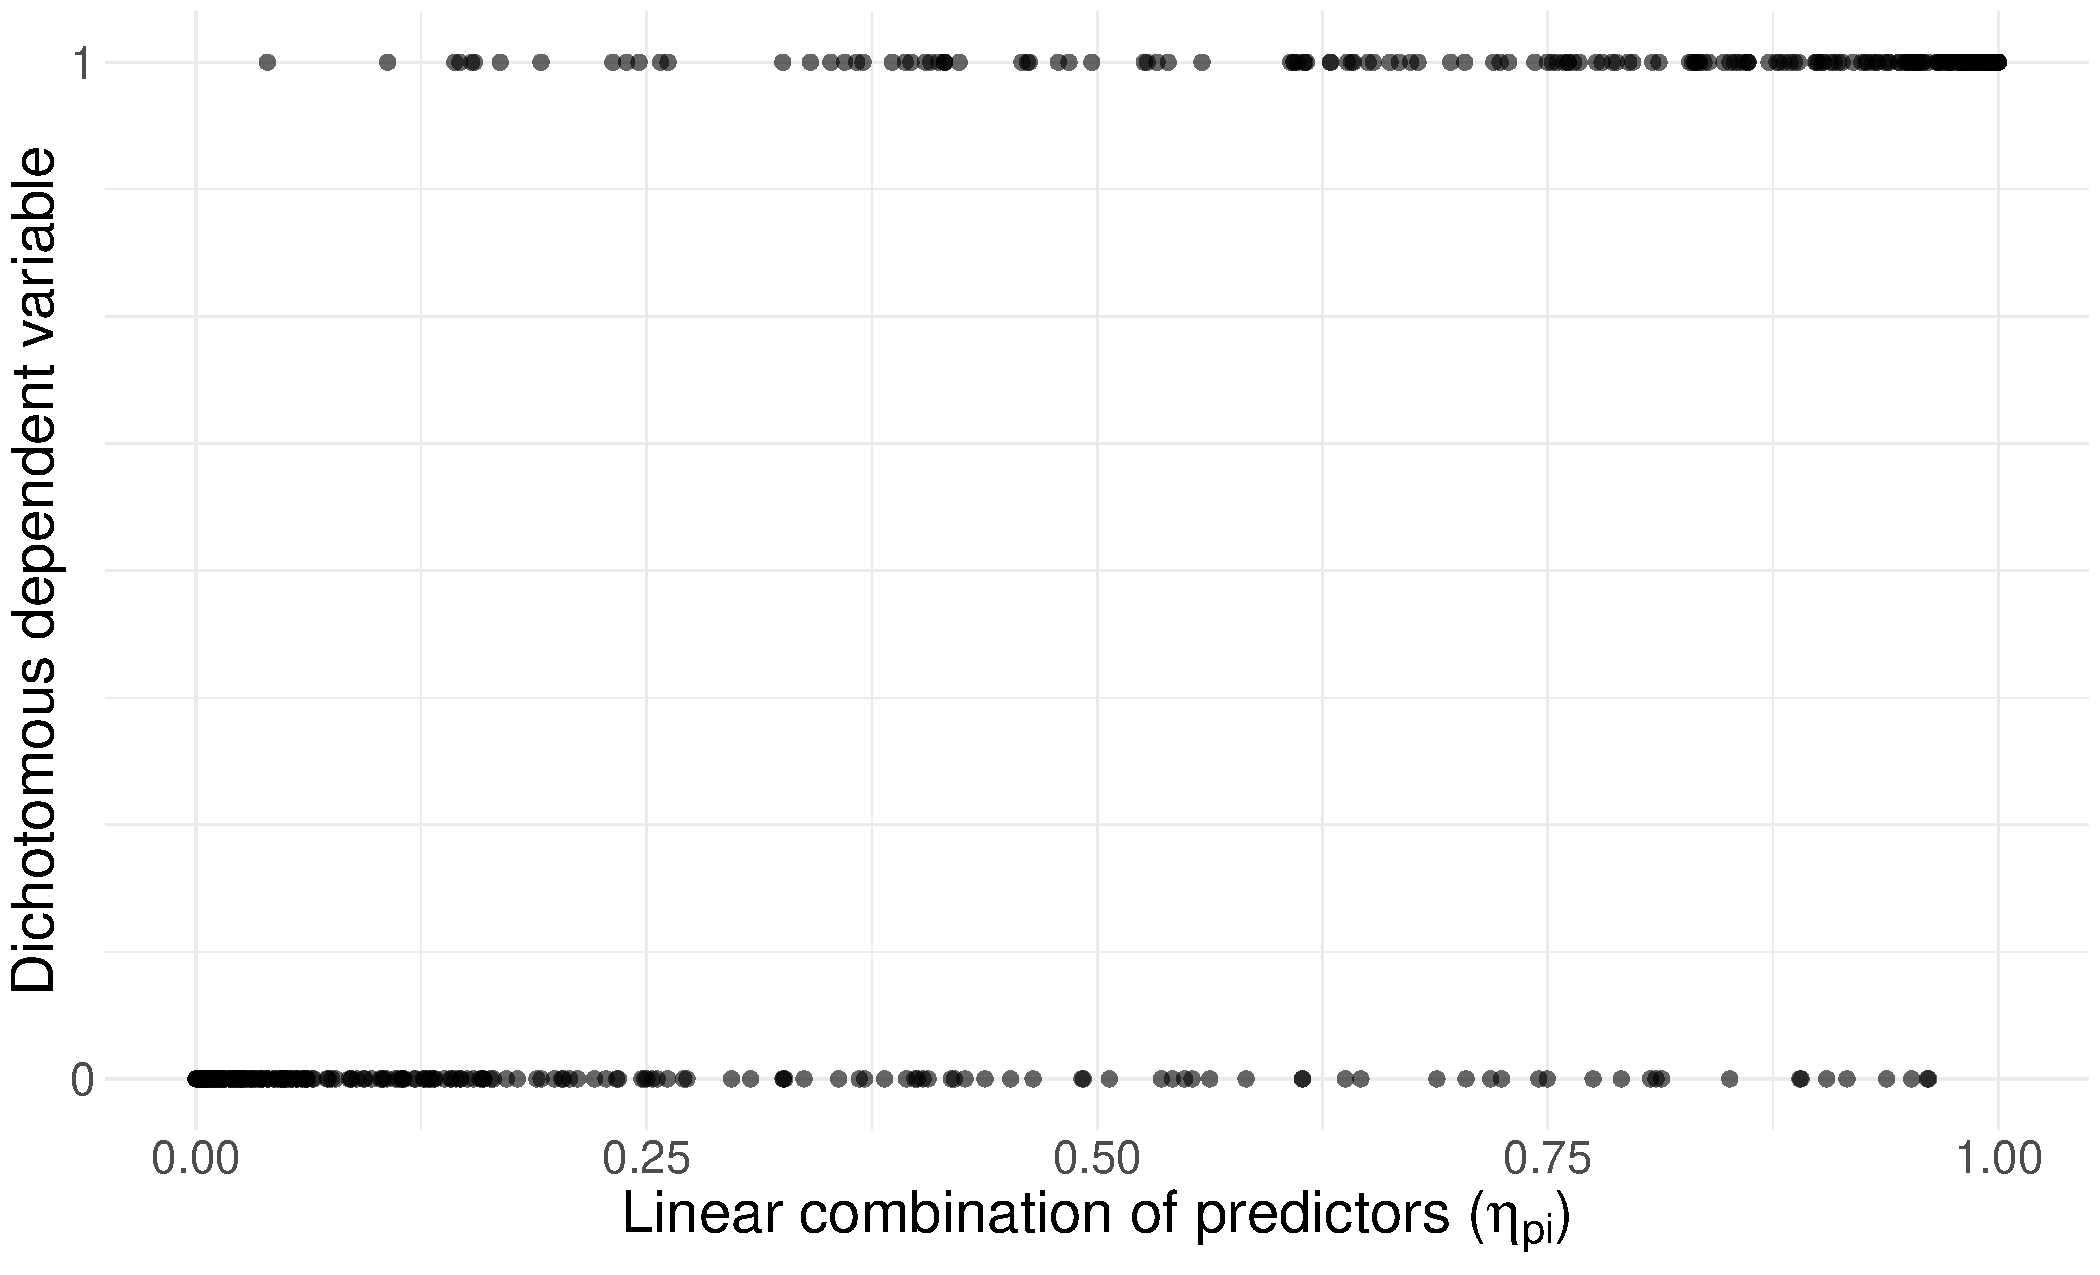
\includegraphics[width=0.7\linewidth]{img/baseGLM.pdf}
			\onslide<2>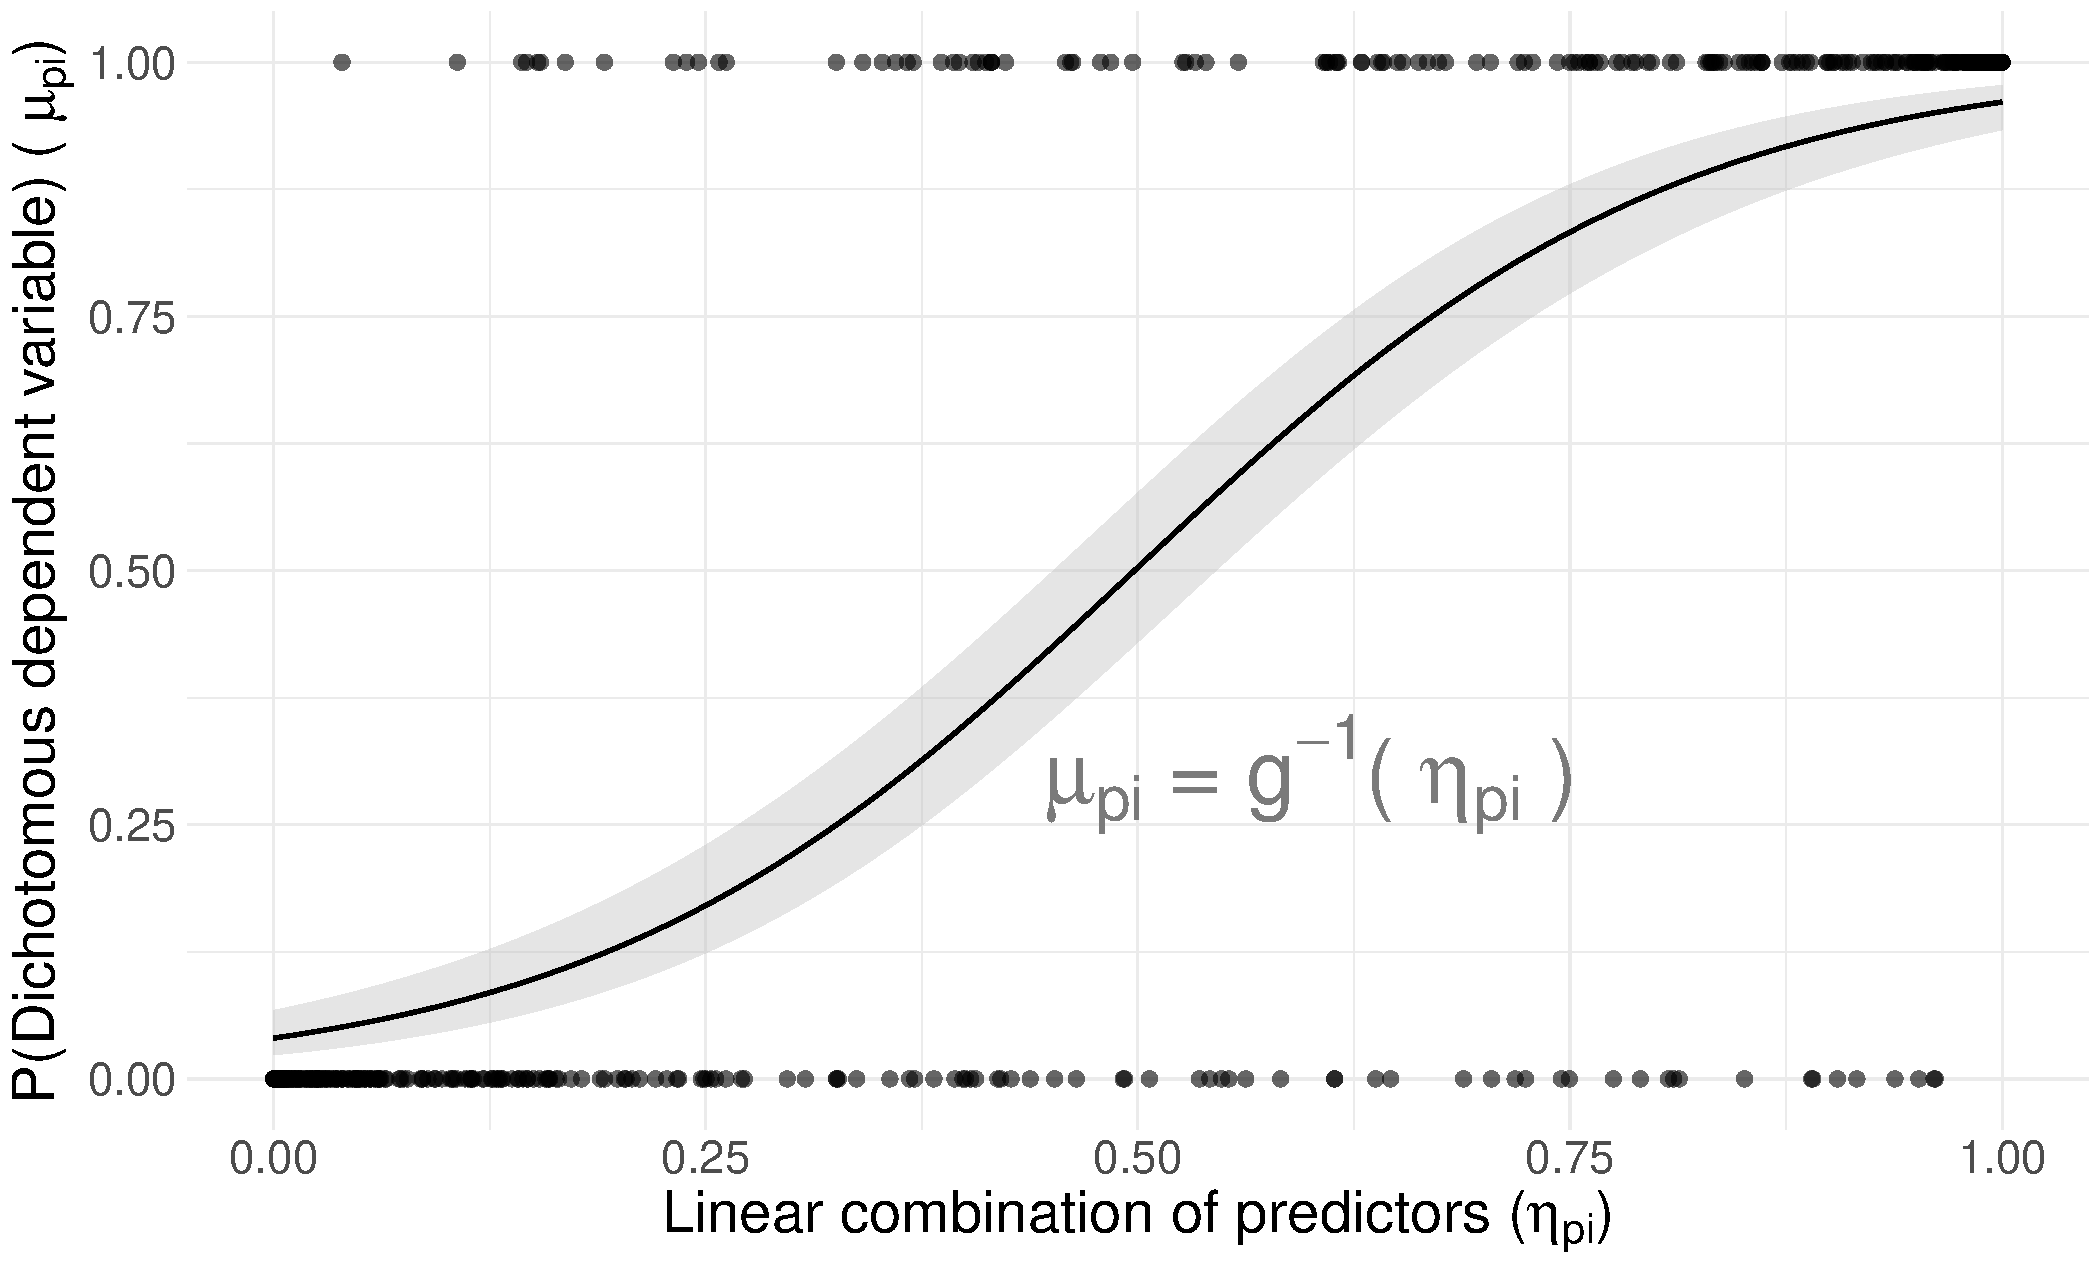
\includegraphics[width=0.7\linewidth]{img/linkGLM.pdf}
		\end{overprint}
	\end{figure}
	
	\onslide<2->
	\tikzoverlay (n1) at (9cm, 5.6cm){%
		\begin{minipage}{0.7\linewidth}
			
			Logit link function $g$:
			
			$g(\eta_{pi}) = log\left(\frac{\mu_{pi}}{1 - \mu_{pi}}\right)$
			
			\vspace{5mm}
			
			Inverse $g^{-1}$
			
			\vspace{5mm}
			
			$g^{-1} = \frac{\exp(\eta_{pi})}{1 + \exp(\eta_{pi})} $
			
			\vspace{1.5mm}
			%	where $\eta_{ps} = \theta_p + b_s$
		\end{minipage}
	}; 
	
\end{frame}



%\begin{frame}{The Rasch model}
%%	\begin{equation*}
%%		P(x_{ps} = 1| \theta_p, b_s) = \dfrac{\exp( \theta_p - b_s)}{1 + \exp(\theta_p - b_s)}
%%	\end{equation*}
%%	where: 
%%	
%%	$\theta_p$: ability of respondent $p$ (i.e., latent trait level of respondent $p$)\\
%%	$b_s$: difficulty of stimulus $s$ (i.e., ``challenging'' power of stimulus $s$)\\
%%	
%%	\vspace{2.5mm}
%%	\onslide<2-> 
%\pause
%\begin{center}
%	Revised
%\end{center}
%	\begin{columns}[T] % align columns
%		\begin{column}{.50\linewidth}
%			\textcolor{diff}{\rule{\linewidth}{2pt}}
%			\begin{center}
%				\textcolor{diff}{	\large{{Standard}}}
%			\end{center}
%			
%		\end{column}
%		
%		\hfill%
%		\begin{column}{.50\linewidth}
%			\textcolor{single}{\rule{\linewidth}{2pt}}
%			\begin{center}
%				\textcolor{single}{\large{{GLM}}}	
%			\end{center}
%			
%		\end{column}%
%	\end{columns}
%	
%	\vspace{2.5mm}
%	\begin{columns}[T]
%		\begin{column}{.50\linewidth}
%			\vspace*{2.5mm}
%			$P(x_{pi} = 1) = \displaystyle \frac{\exp(\theta_p \spot<2->[fill=rasch!50]{-} b_i)}{1 + \exp(\theta_p \spot<2->[fill=rasch!50]{-} b_i)}$
%		\end{column}
%		\hfill
%		
%		\begin{column}{.50\linewidth}
%			
%			
%			\vspace*{2.5mm}
%			$P(x_{ps} = 1) = \displaystyle \frac{\exp(\theta_p \, \spot<2->[fill=single!50]{+} \, b_s)}{1 + \exp(\theta_p \, \spot<2->[fill=single!50]{+} \, b_s)}$
%		\end{column}
%	\end{columns}	
%	
%	
%	\vspace{5mm}
%
%\pause
%\begin{center}
%	Beyond
%\end{center}
%
%\pause
%
%\begin{columns}[T] % align columns
%	\begin{column}{.50\linewidth}
%		\textcolor{diff}{\rule{\linewidth}{2pt}}
%		\begin{center}
%			\textcolor{diff}{	\large{{Log-normal model}}}
%		\end{center}
%		
%	\end{column}
%	
%	\hfill%
%	\begin{column}{.50\linewidth}
%		\textcolor{single}{\rule{\linewidth}{2pt}}
%		\begin{center}
%			\textcolor{single}{\large{{Linear model}}} 	
%		\end{center}
%		
%	\end{column}%
%\end{columns}
%
%\vspace{2.5mm}
%\begin{columns}[T]
%	\begin{column}{.50\linewidth}
%		\centering
%		\vspace*{2.5mm}
%		$f (t_{ps}) =  \delta_i \, \spot<4->[fill=log!50]{-} \, \tau_p \, + \, \varepsilon $
%	\end{column}
%	\hfill
%	
%	\begin{column}{.50\linewidth}
%		\centering
%		\vspace*{2.5mm}
%		$f(t_{ps}) =  \delta_i \, \spot<4->[fill=log!50]{+} \, \tau_p \, +  \, \varepsilon$
%	\end{column}
%\end{columns}
%
%\end{frame}


\begin{frame}{Random effects and random factors}
	Linear combination of predictors in a Linear Model: 
	\begin{equation*}
		\eta = X \beta,
	\end{equation*}
	where $\beta$ indicates the coefficients of the fixed intercept and slope(s), and $X$ is the model-matrix.
	

	Linear combination of predictors in a Linear Mixed-Effects Model (LMM): 
	
	\begin{equation*}
		\eta = X \beta + Zd,
	\end{equation*}
	where $Z$ is the matrix and $d$ is the vector of the random effects (not parameters!)
	
	
	\vspace{2.5mm}
	\begin{center}
		\emph{Best Linear Unbiased Predictors}
	\end{center}
\end{frame}

\begin{frame}
	\centering
		\scalebox{.50}{
			\begin{tikzpicture}[inner sep=1pt,auto=left, node distance=2cm,>=latex']
			
			\node(s1) at(2, 16)  [respondent]  {$p_1$};
			\node(s2) at (2, 11) [respondent] {$p_2$};
			\node(s3) at (2, 5.5) [respondent] {$p_3$};
			\node(t1) at (12, 17) [ trial] {};
			\node(t2) at (12, 15.5) [trial] {};
			\node(t3) at (12, 14) [trial] {};
			\node(t4) at (12, 12.5) [trial] {};
			\node(t5) at (12, 9) [trial] {};
			\node(t6) at (12, 7.5) [trial] {};
			\node(t7) at (12, 6) [trial] {};
			\node(t8) at (12, 4.5) [trial] {};
			\node(stim1) at(22, 13)  [stimulus]  {\Smiley[3]};
			\node(stim2) at (22, 7) [stimulus] {\Sleepey[3]};
			\node at (12, 14.8) [condition, dashed,ultra thick] {};  
			\node at (12, 6.8) [condition, black,ultra thick] {};  
			\draw [->, shorten >= +3pt] (s1.east) -- (t1.west);
			\draw [->, shorten >= +3pt] (s2.east) -- (t1.west);
			\draw [->, shorten >= +3pt] (s3.east) -- (t1.west);
			\draw [->, shorten >= +3pt] (s1.east) -- (t2.west);
			\draw [->, shorten >= +3pt] (s2.east) -- (t2.west);
			\draw [->, shorten >= +3pt] (s3.east) -- (t2.west);
			\draw [->, shorten >= +3pt] (s1.east) -- (t3.west);
			\draw [->, shorten >= +3pt] (s2.east) -- (t3.west);
			\draw [->, shorten >= +3pt] (s3.east) -- (t3.west);
			\draw [->, shorten >= +3pt] (s1.east) -- (t4.west);
			\draw [->, shorten >= +3pt] (s2.east) -- (t4.west);
			\draw [->, shorten >= +3pt] (s3.east) -- (t4.west);
			\draw [->, shorten >= +3pt] (s1.east) -- (t5.west);
			\draw [->, shorten >= +3pt] (s2.east) -- (t5.west);
			\draw [->, shorten >= +3pt] (s3.east) -- (t5.west);
			\draw [->, shorten >= +3pt] (s1.east) -- (t6.west);
			\draw [->, shorten >= +3pt] (s2.east) -- (t6.west);
			\draw [->, shorten >= +3pt] (s3.east) -- (t6.west);
			\draw [->, shorten >= +3pt] (s1.east) -- (t7.west);
			\draw [->, shorten >= +3pt] (s2.east) -- (t7.west);
			\draw [->, shorten >= +3pt] (s3.east) -- (t7.west);
			\draw [->, shorten >= +3pt] (s1.east) -- (t8.west);
			\draw [->, shorten >= +3pt] (s2.east) -- (t8.west);
			\draw [->, shorten >= +3pt] (s3.east) -- (t8.west);
			\draw [<-, shorten <= +3pt] (t1.east)  -- (stim1.west); 
			\draw [<-, shorten <= +3pt] (t2.east)  -- (stim2.west); 
			\draw [<-, shorten <= +3pt] (t3.east)  -- (stim1.west); 
			\draw [<-, shorten <= +3pt] (t4.east)  -- (stim2.west); 
			\draw [<-, shorten <= +3pt] (t5.east)  -- (stim1.west); 
			\draw [<-, shorten <= +3pt] (t6.east)  -- (stim2.west); 
			\draw [<-, shorten <= +3pt] (t7.east)  -- (stim1.west); 
			\draw [<-, shorten <= +3pt] (t8.east)  -- (stim2.west); 
		\end{tikzpicture}
		}

\end{frame}



\begin{frame}{}
	
	
	\begin{block}{Generalizability}
		
		\small
		
		Generalizability is bounded to the specific set of stimuli used in the experiment
		
		Results can be generalized if and only if the exact same set of stimuli is used 
		
		
	\end{block}
	
	
	\begin{block}{Robustness of the results}
		
		\small
		Random variability at the stimulus level might inflate the probability of committing Type I errors
		
		Averaging across stimuli to obtain person-level scores results in biased estimates due to the noise in the data
	\end{block}
	
	
	\begin{block}{Loss of information}
		
		\small
		
		All the variability is not considered as well as all the information that can be obtained from it 
		
		Every stimulus is assumed to be equally informative
	\end{block}
	
\end{frame}

\section[IRT and short test forms]{Item Response Theory \\and short test forms development}



%\begin{frame}{Aim}
%	\tikzoverlay (n1) at (0.2cm,1.3cm) {%
%		\begin{minipage}{\textwidth}%
%			\begin{block}{}%
%				\centering{\large{New IRT-based procedures for shortening tests}}
%				
%				\vspace{3mm}
%				
%			\end{block}
%		\end{minipage}
%	};%
%	\onslide<2->
%	\tikzoverlay (n2) at (-1cm,-0.5cm) {%
%		\begin{minipage}{0.6\textwidth}%
%			\begin{block}{}%
%				\centering
%				Equal for all respondents 
%			\end{block}
%		\end{minipage}
%	};%
%	\onslide<3->
%	\tikzoverlay (n3) at (5.6cm,-0.5cm) {%
%		\begin{minipage}{0.6\textwidth}%
%			\begin{block}{}%
%				\centering
%				Tailored to specific levels of \\ the latent trait
%			\end{block}
%		\end{minipage}
%	};%
%	%
%	
%	\begin{tikzpicture}[remember picture, overlay]
%		\onslide<2->  \path [line width=0.04cm,->,shorten >= +3pt, template] (n1.south) edge (n2.north);
%		\onslide<3->  \path [line width=0.04cm,->, shorten >= +3pt, template] (n1.south)  edge (n3.north);
%	\end{tikzpicture}
%	
%\end{frame}




\begin{frame}{2-Parameter Logistic Model}

%\color{blue}mi sono costate sangue ma queste saltano \normalcolor

\centering
\begin{overprint}

\centering
	\onslide<1>
		\vspace*{1mm}
		
Item Response Function:	$P(x_{pi} = 1|\theta_p, b_i, a_i) = \frac{\exp[a_j(\theta_p - b_i)]}{1 + \exp[a_j(\theta_p - b_i)]}$
	
\vspace{1.5mm}
	\centering
	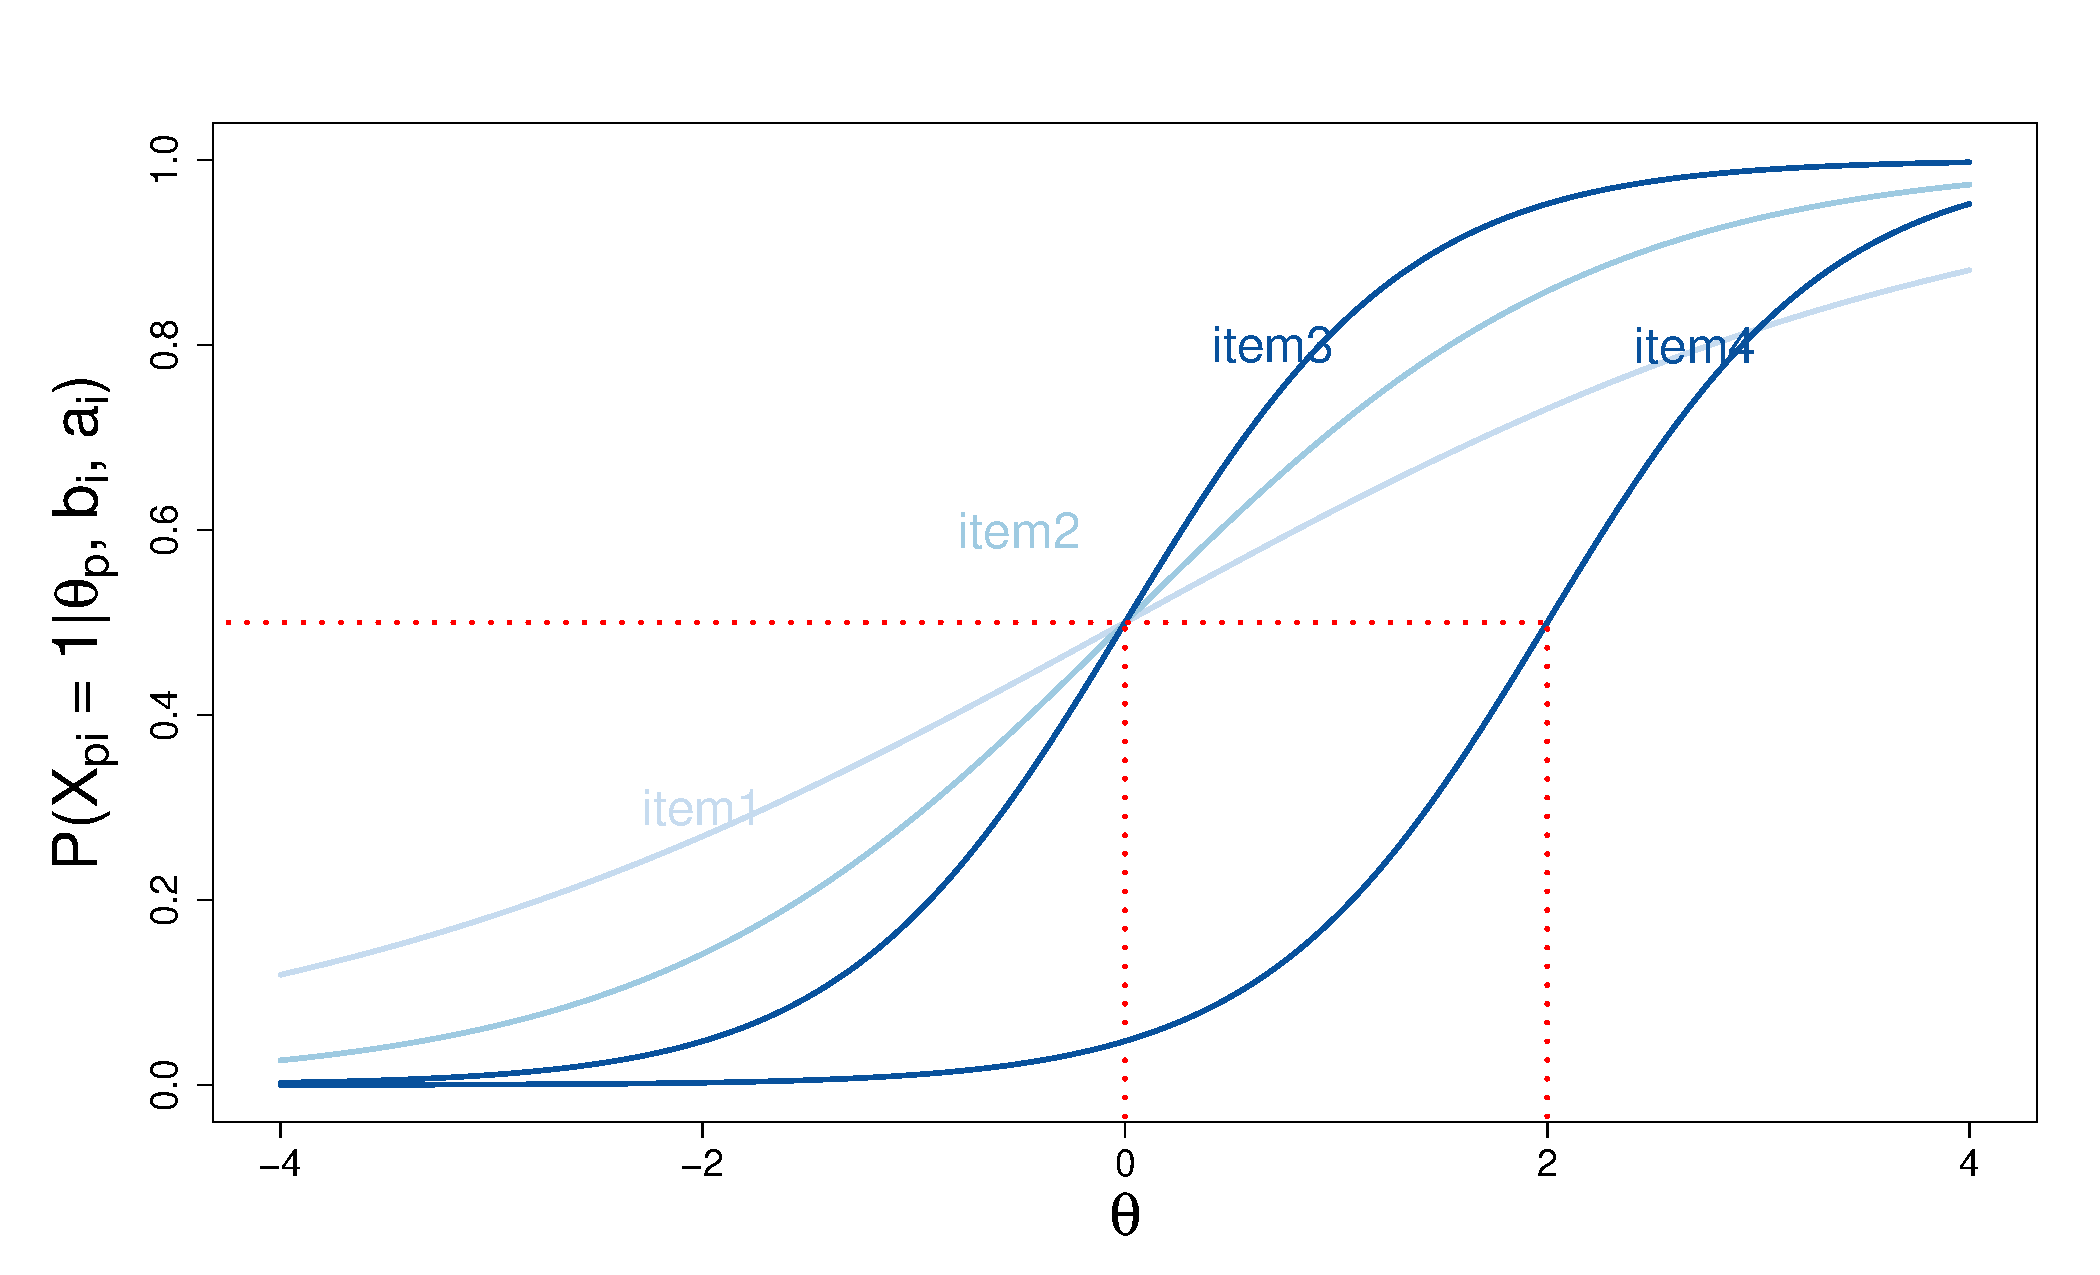
\includegraphics[width=.70\linewidth]{img/ICC-2pl.pdf}
	
	\onslide<2>
		\vspace*{3mm}
		
Item Information Function:	$I_i(\theta) = a_i^2P_(\theta, b_i, a_i)[1-P_i(\theta, b_i, a_i)]$
	
	\centering
	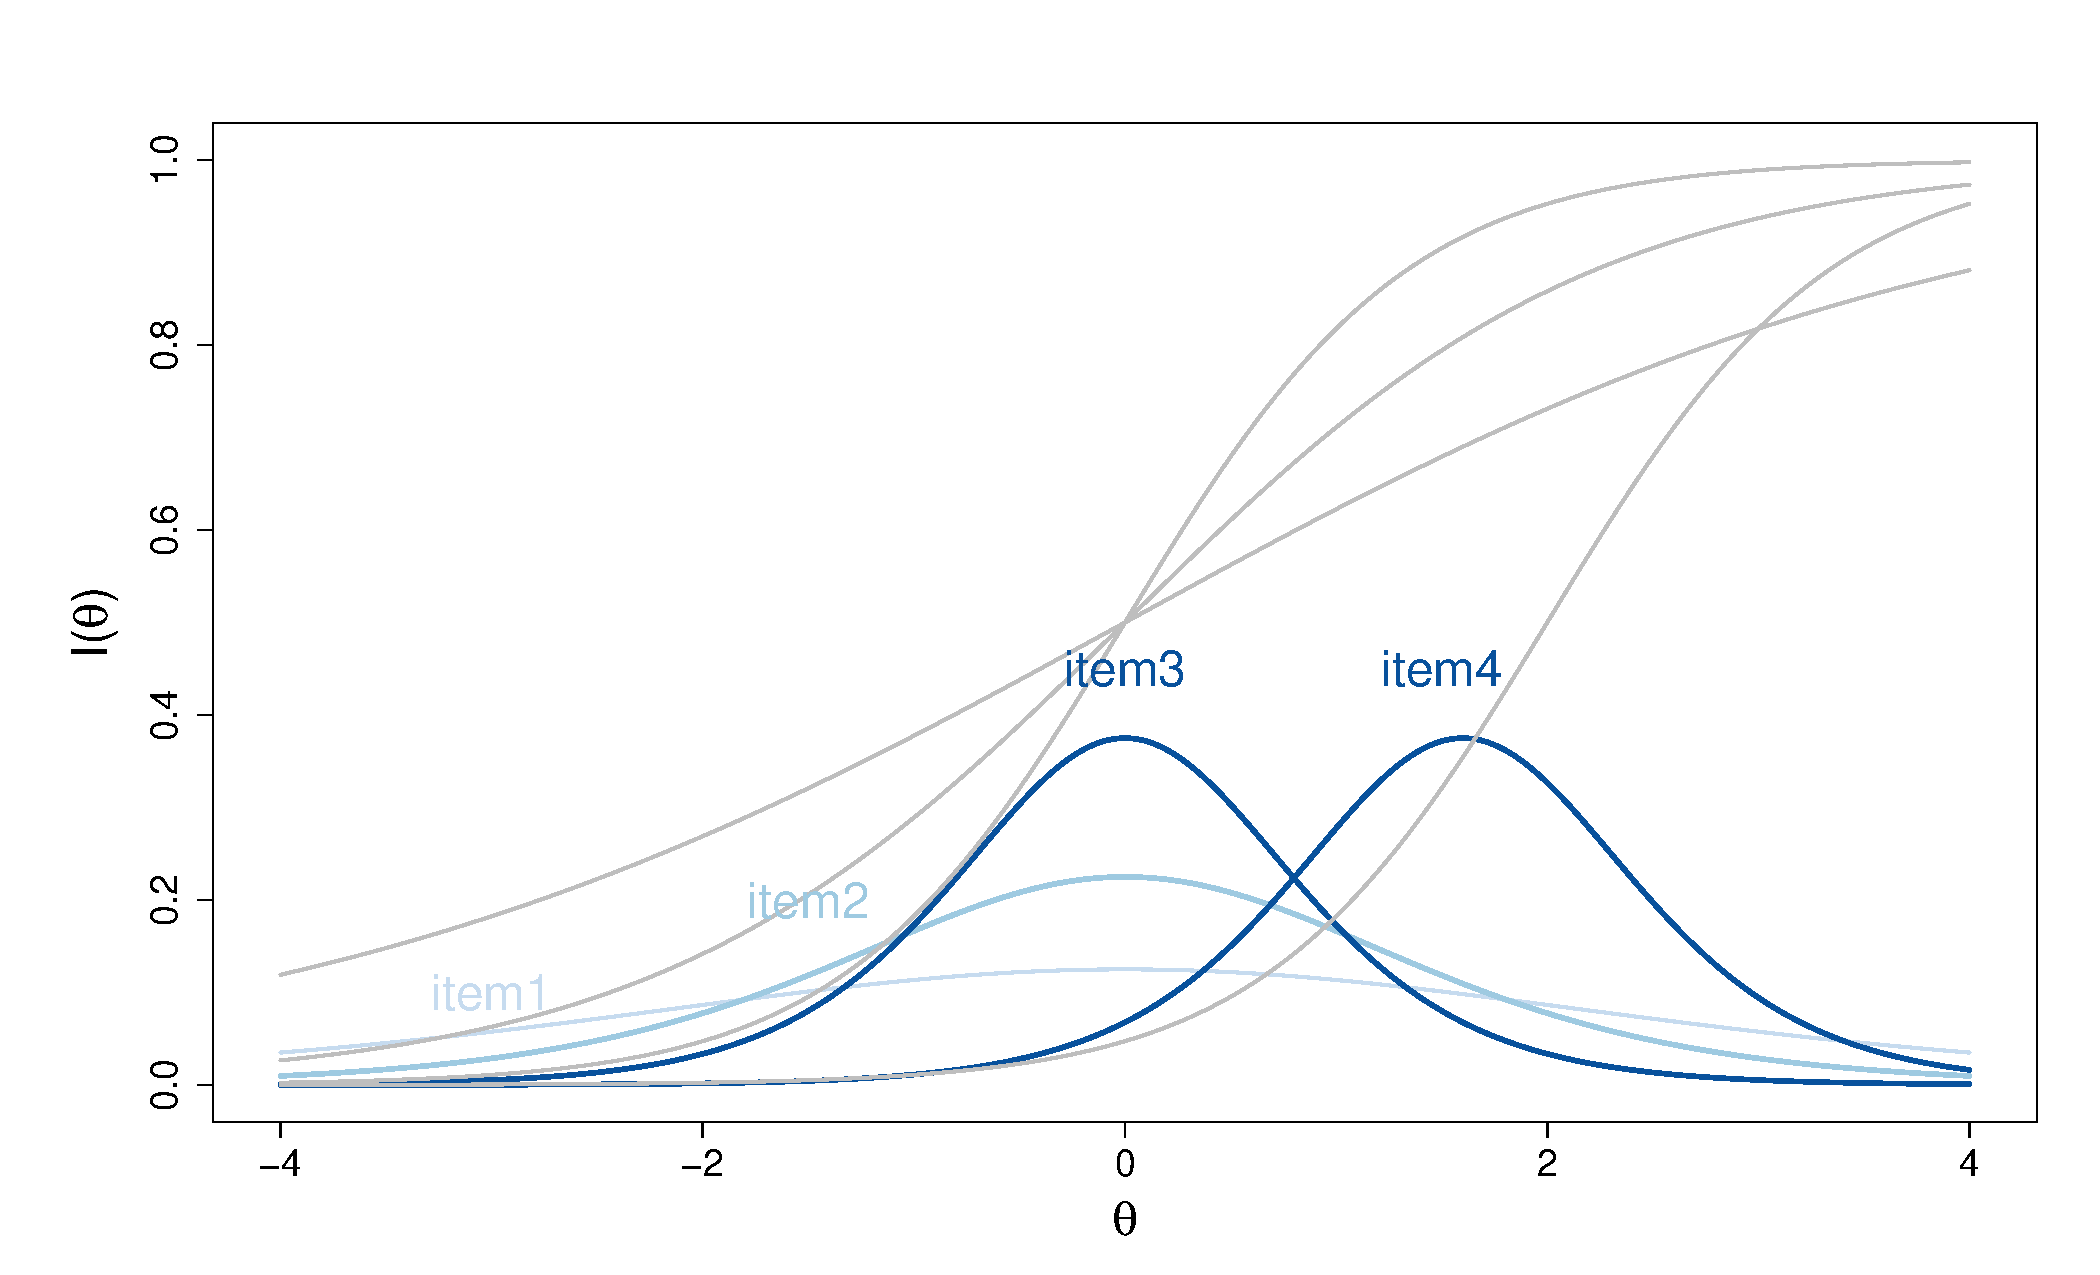
\includegraphics[width=.70\linewidth]{img/IIF-2pl.pdf}
	
		\onslide<3>
		\vspace*{3mm}
Test Information Function:		$I(\theta) =  \sum_{i = 1}^{I} I_i(\theta)$
	
	\centering
	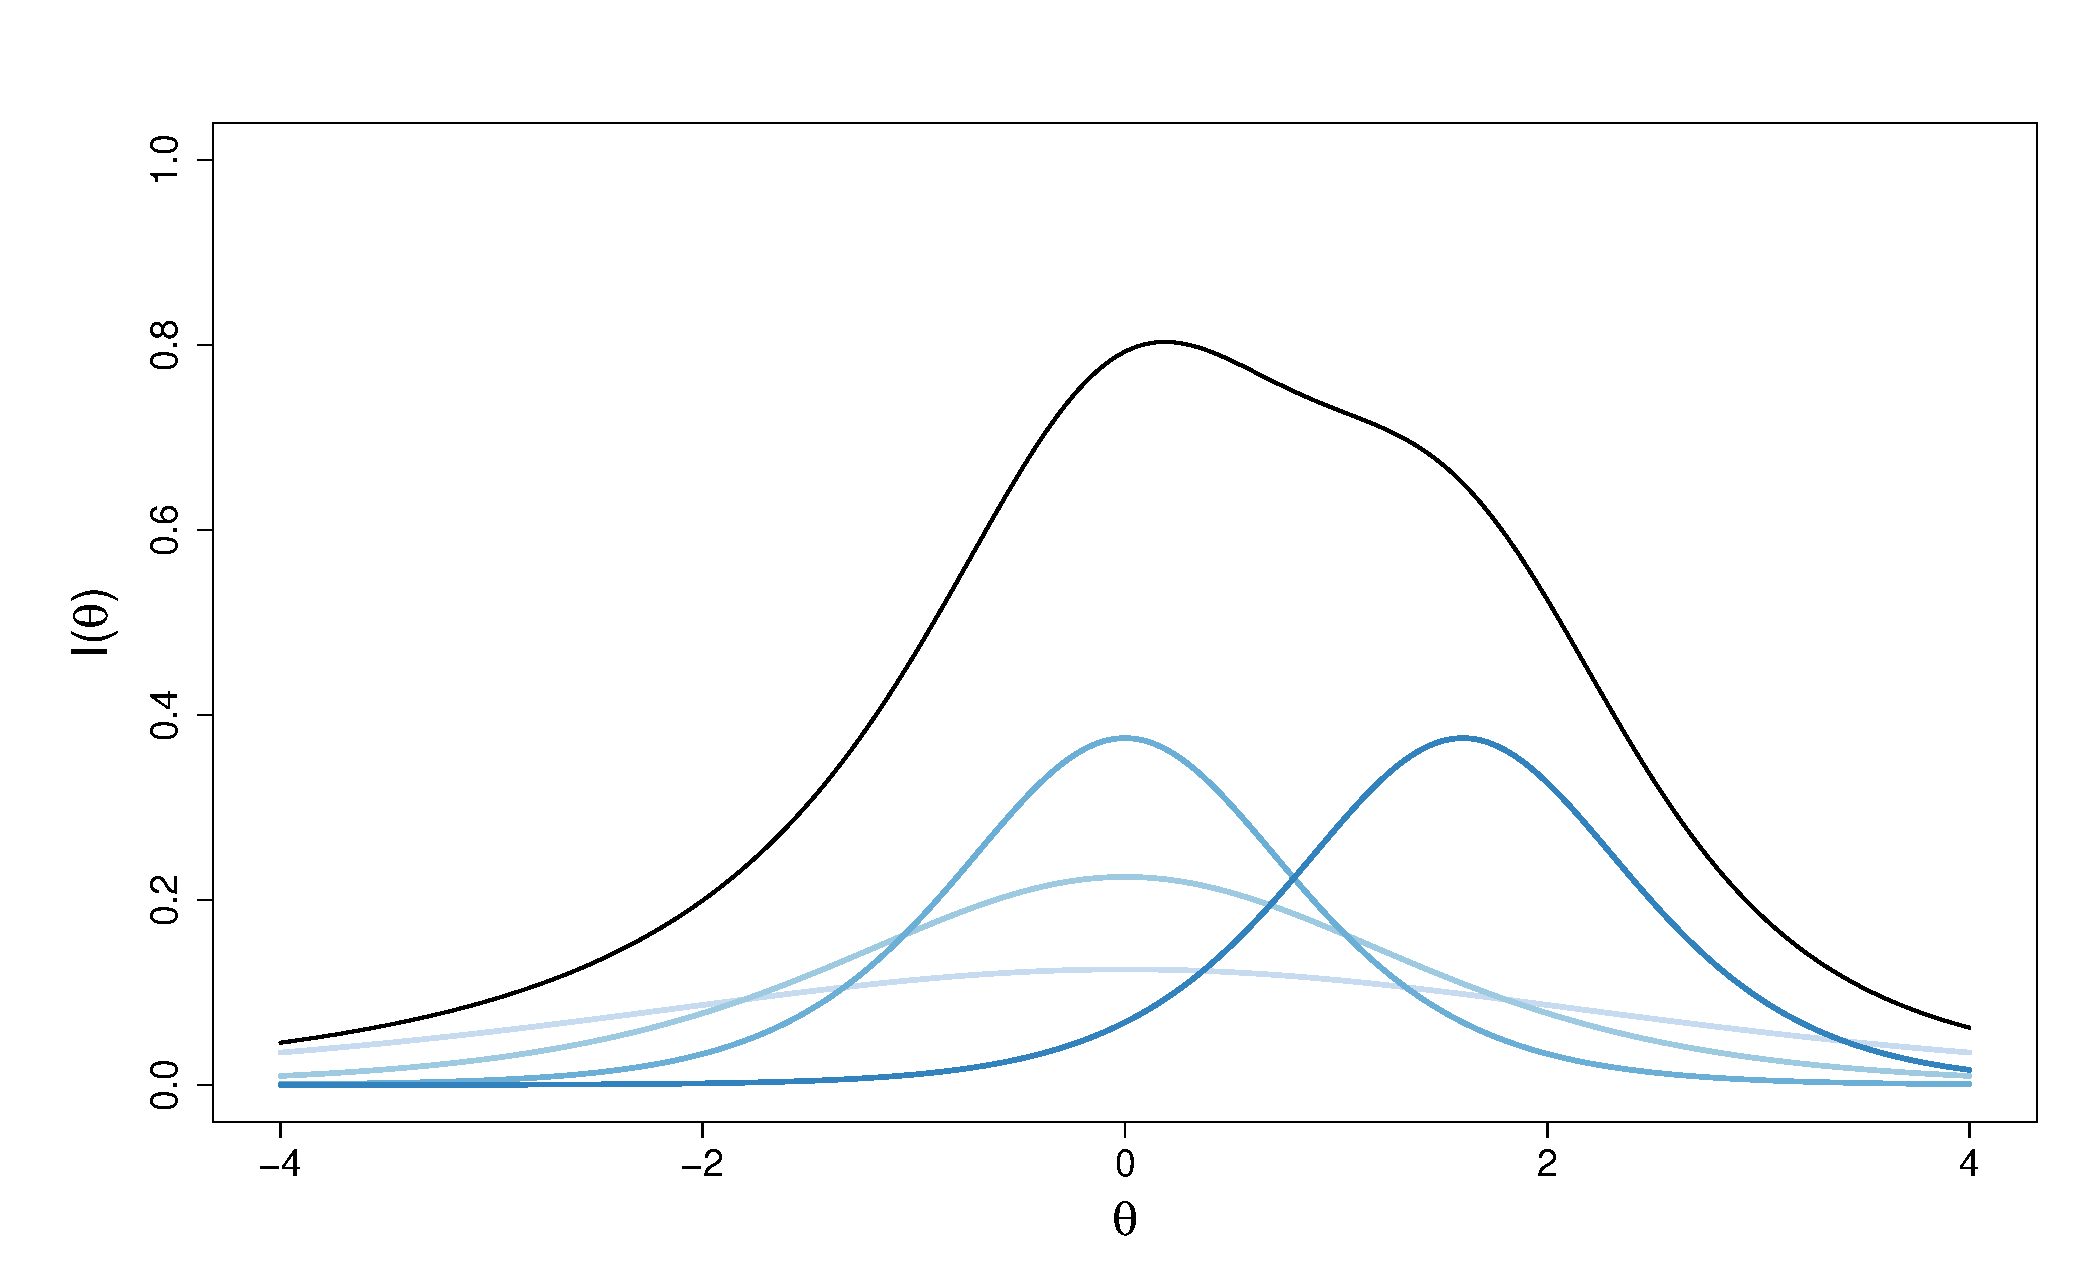
\includegraphics[width=.70\linewidth]{img/TIF-2pl.pdf}
\end{overprint}
			
	
	
	
\end{frame}

%\begin{frame}{Item Response Theory and short test forms}
%	
%	\textbf{\textsc{\textcolor{black}{Adaptive short forms}}}: \emph{Ad-hoc} tests for each person \textcolor{template}{$\rightarrow$} The information is maximized for each level of $\theta$ (i.e., for each respondent) \textcolor{template}{$\rightarrow$} (\textcolor{template}{\textbf{CAT}}: Computerized Adaptive Testing)
%	
%	\onslide<2->
%	\begin{block}{Issue}
%		
%		Different short test forms for each respondent $\rightarrow$ Potential fairness issues in assessments, e.g. for recruitment
%	\end{block}
%	
%	\onslide<1->
%	\textbf{\textcolor{black}{\textsc{Static short forms}}}: Static tests equal for all respondents \textcolor{template}{$\rightarrow$} The information is maximized across $\theta$ levels (i.e., across all respondents)
%	
%	\onslide<3->
%	\begin{block}{Issue}
%		
%		Not being tailored to any $\theta$ level of interest \textcolor{template}{$\rightarrow$} Potentially more items are needed to  cover a wide range of $\theta$s
%	\end{block}
%	
%	
%\end{frame}

\begin{frame}{$\theta$-target procedures}
	Selected items $\rightarrow$ items with highest \emph{IIF}s in respect to $\theta$ targets ($\theta'$) 
	
	\begin{quote}
		\small
		e.g.:	3-item short form from 10-item full-length test
	\end{quote}
	\vspace*{-5mm}
	\begin{overprint}
		\small
		\onslide<1>
		\begin{table}
			\begin{tabular}{l l l l }
				\toprule
				& \multicolumn{1}{c}{$\theta_1'$} & \multicolumn{1}{c}{$\theta_2'$} & \multicolumn{1}{c}{ $\theta_3'$} \\
				item	& $	-2.67	$ & $	0.01	$ & $	2.67	$ \\
				\midrule
				1	& & & \\
				2	&  & & 	\\
				3	&  &  &  \\
				4&  & & \\
				5	&  & & 	 \\
				6	&  & &  \\
				7	& & &  \\
				8	& & &  \\
				9	& &  &  \\
				10	&& & 	 \\
				\bottomrule
			\end{tabular}
		\end{table}
		\onslide<2->
		\begin{table}
			\begin{tabular}{l l l l }
				\toprule
				& \multicolumn{1}{c}{\textcolor<3->{orangered2}{$\theta_1'$}} & \multicolumn{1}{c}{\textcolor<7->{springgreen}{$\theta_2'$}} & \multicolumn{1}{c}{ \textcolor<5->{diff}{$\theta_3'$}} \\
				item	& \textcolor<3->{orangered2}{$	-2.67	$} & \textcolor<7->{springgreen}{$	0.01	$} & \textcolor<5->{diff}{$	2.67	$} \\
				\midrule
				1	& \textcolor<4->{black!30}{$	0.04	$} & \textcolor<8->{black!30}{$	0.12	$} & 	\textcolor<6->{black!30}{$	0.08	$} \\
				\textcolor<8->{black!30 }{2}	& \textcolor<4->{black!30}{$	0.09	$} & \textcolor<7->{springgreen}{$	0.33	$} & 	\textcolor<6->{black!30}{$	0.03	$} \\
				3	& \textcolor<4->{black!30}{$	0.01	$} & \textcolor<8->{black!30}{$	0.01	$} & 	\textcolor<6->{black!30}{$	0.02	$} \\
				\textcolor<4->{black!30}{4}	& \textcolor<3->{orangered2}{$	0.73	$} & \textcolor<4->{black!30}{$	0.06	$} & \textcolor<4->{black!30}{$	0.01	$} \\
				5	& \textcolor<4->{black!30}{$	0.04	$} & \textcolor<8->{black!30}{$	0.03	$} & 	\textcolor<6->{black!30}{$	0.02	$} \\
				6	& \textcolor<4->{black!30}{$	0.01	$} & \textcolor<8->{black!30}{$	0.06	$} & 	\textcolor<6->{black!30}{$	0.59	$} \\
				7	& \textcolor<4->{black!30}{$	0.05	$} & \textcolor<8->{black!30}{$	0.06	$} & 	\textcolor<6->{black!30}{$	0.03	$} \\
				\textcolor<6->{black!30}{8}	& \textcolor<4->{black!30}{$	0.01	$} & 	\textcolor<6->{black!30}{$	0.04	$} & \textcolor<5->{diff}{$	0.69	$} \\
				9	& \textcolor<4->{black!30}{$	0.03	$} & \textcolor<8->{black!30}{$	0.05	$} & 	\textcolor<6->{black!30}{$	0.04	$} \\
				10	& \textcolor<4->{black!30}{$	0.02	$} & \textcolor<8->{black!30}{$	0.03	$} & 	\textcolor<6->{black!30}{$	0.02	$} \\
				\bottomrule
			\end{tabular}
		\end{table}
		
	\end{overprint}
	
	
	
\end{frame}


\begin{frame}{The other way around}


\begin{overprint}
	\centering
	\onslide<1>
	\centering
	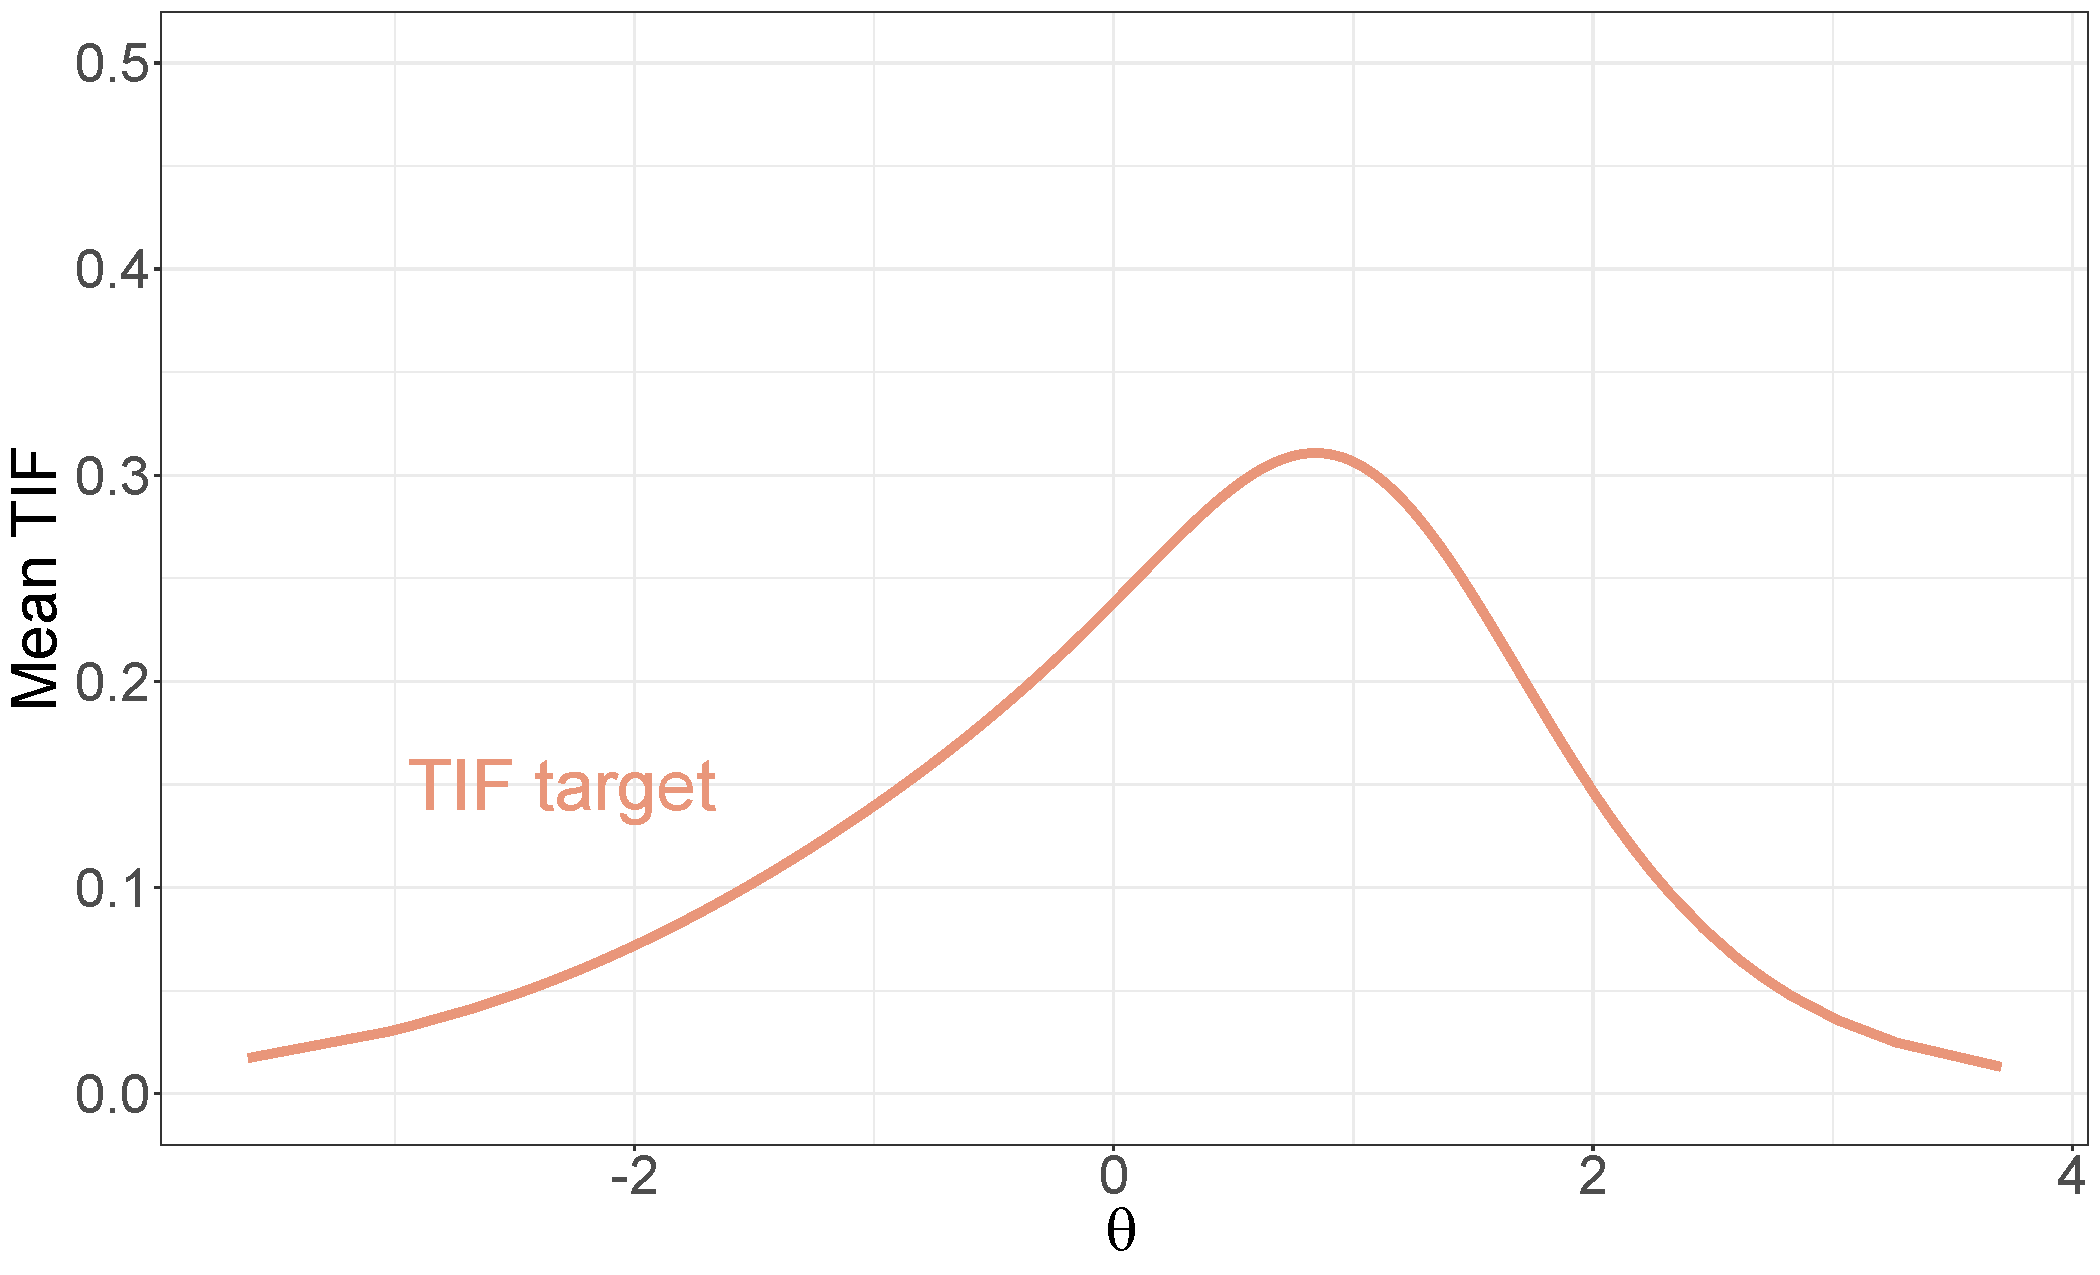
\includegraphics[width=.80\textwidth]{img/TIF-target.pdf}
	
	\onslide<2>
	\centering
	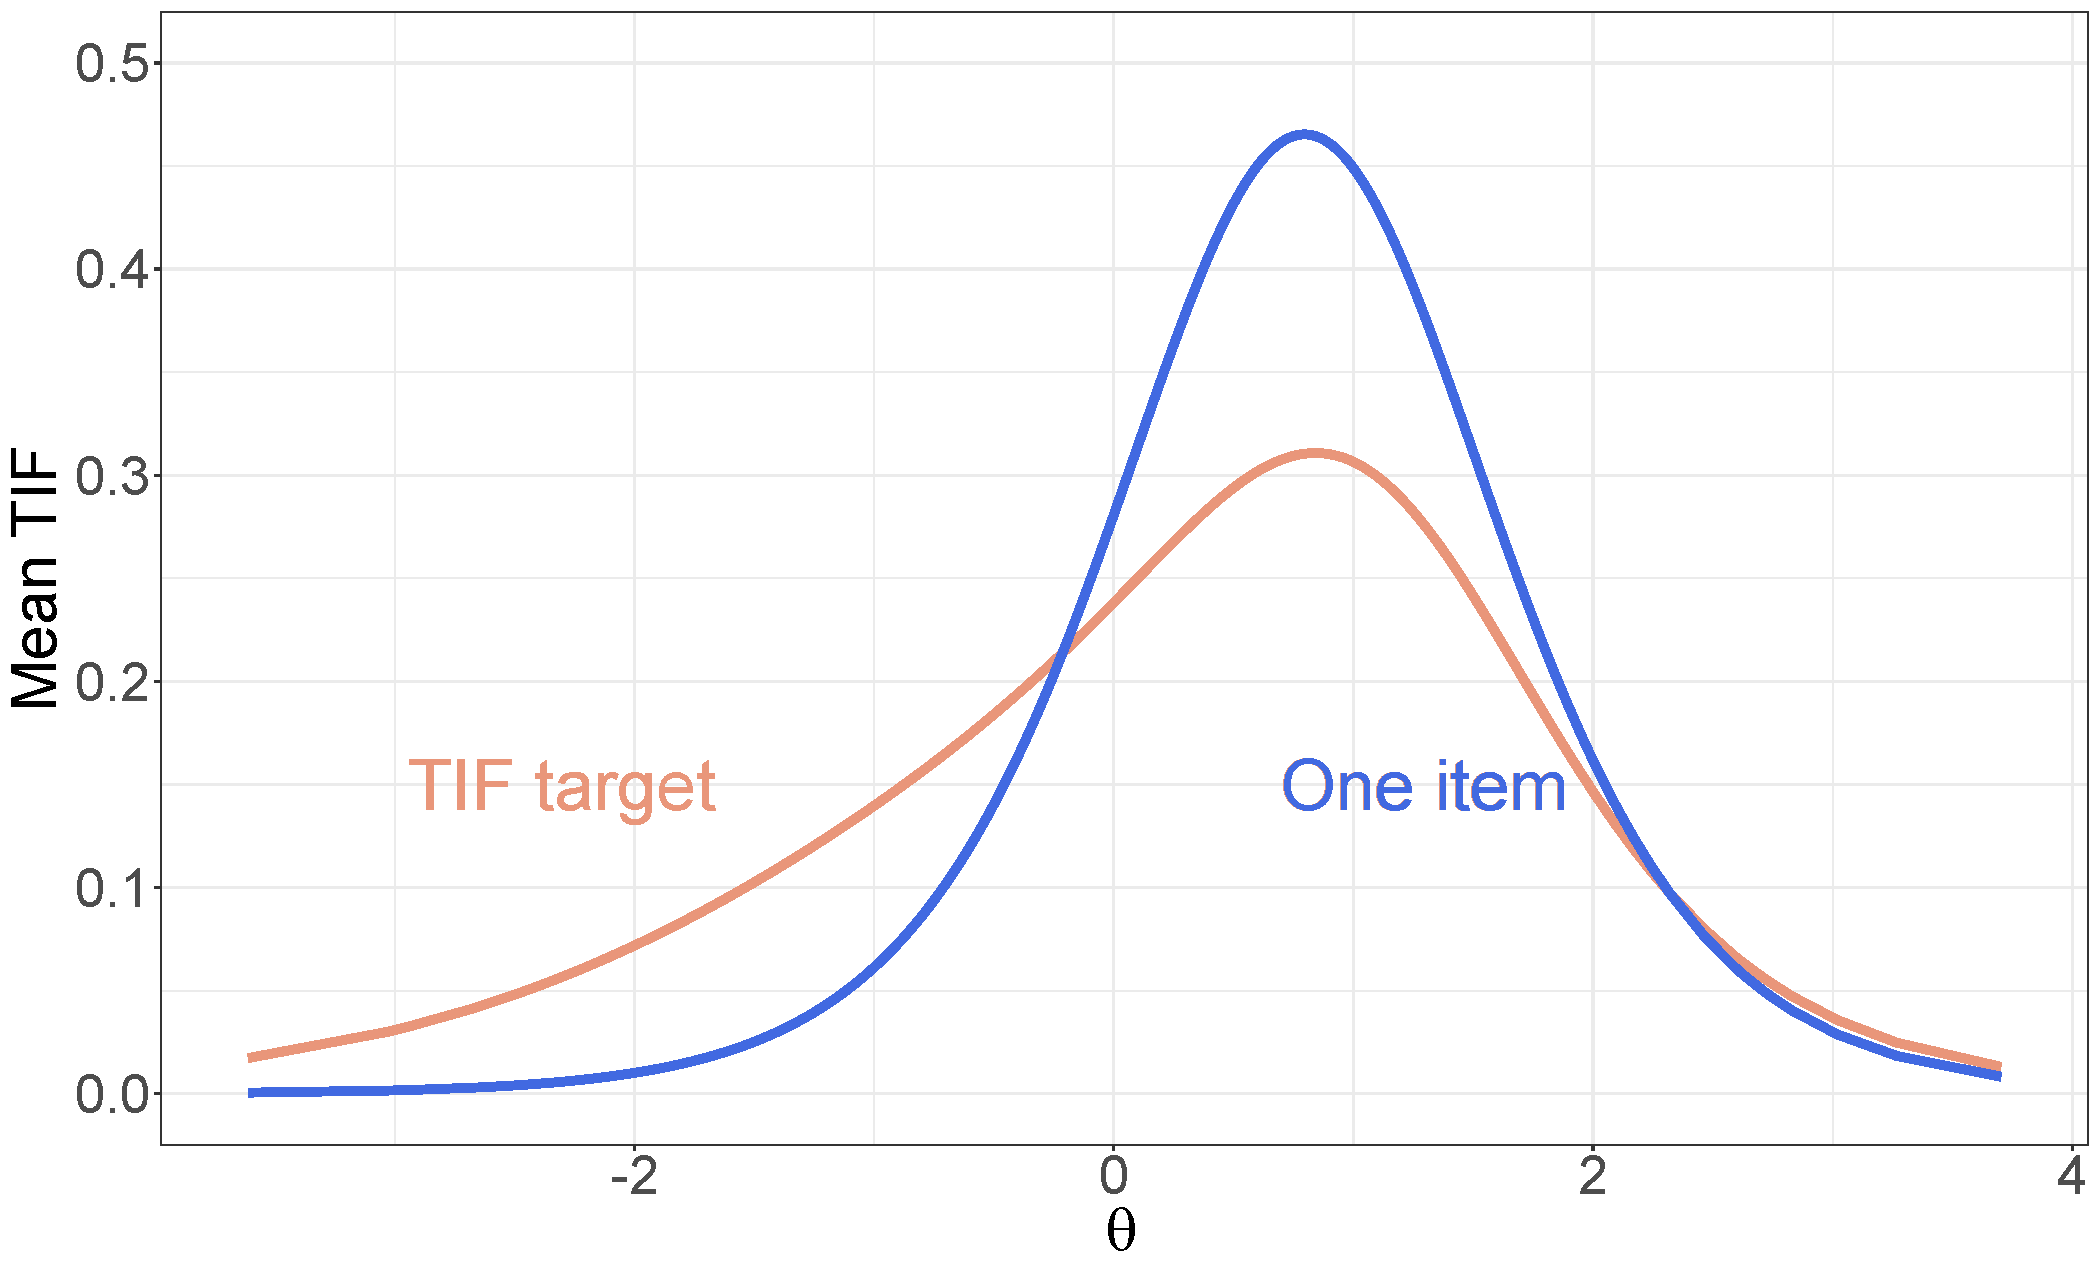
\includegraphics[width=.80\textwidth]{img/TIF-first.pdf}
	
	\onslide<3>\centering
	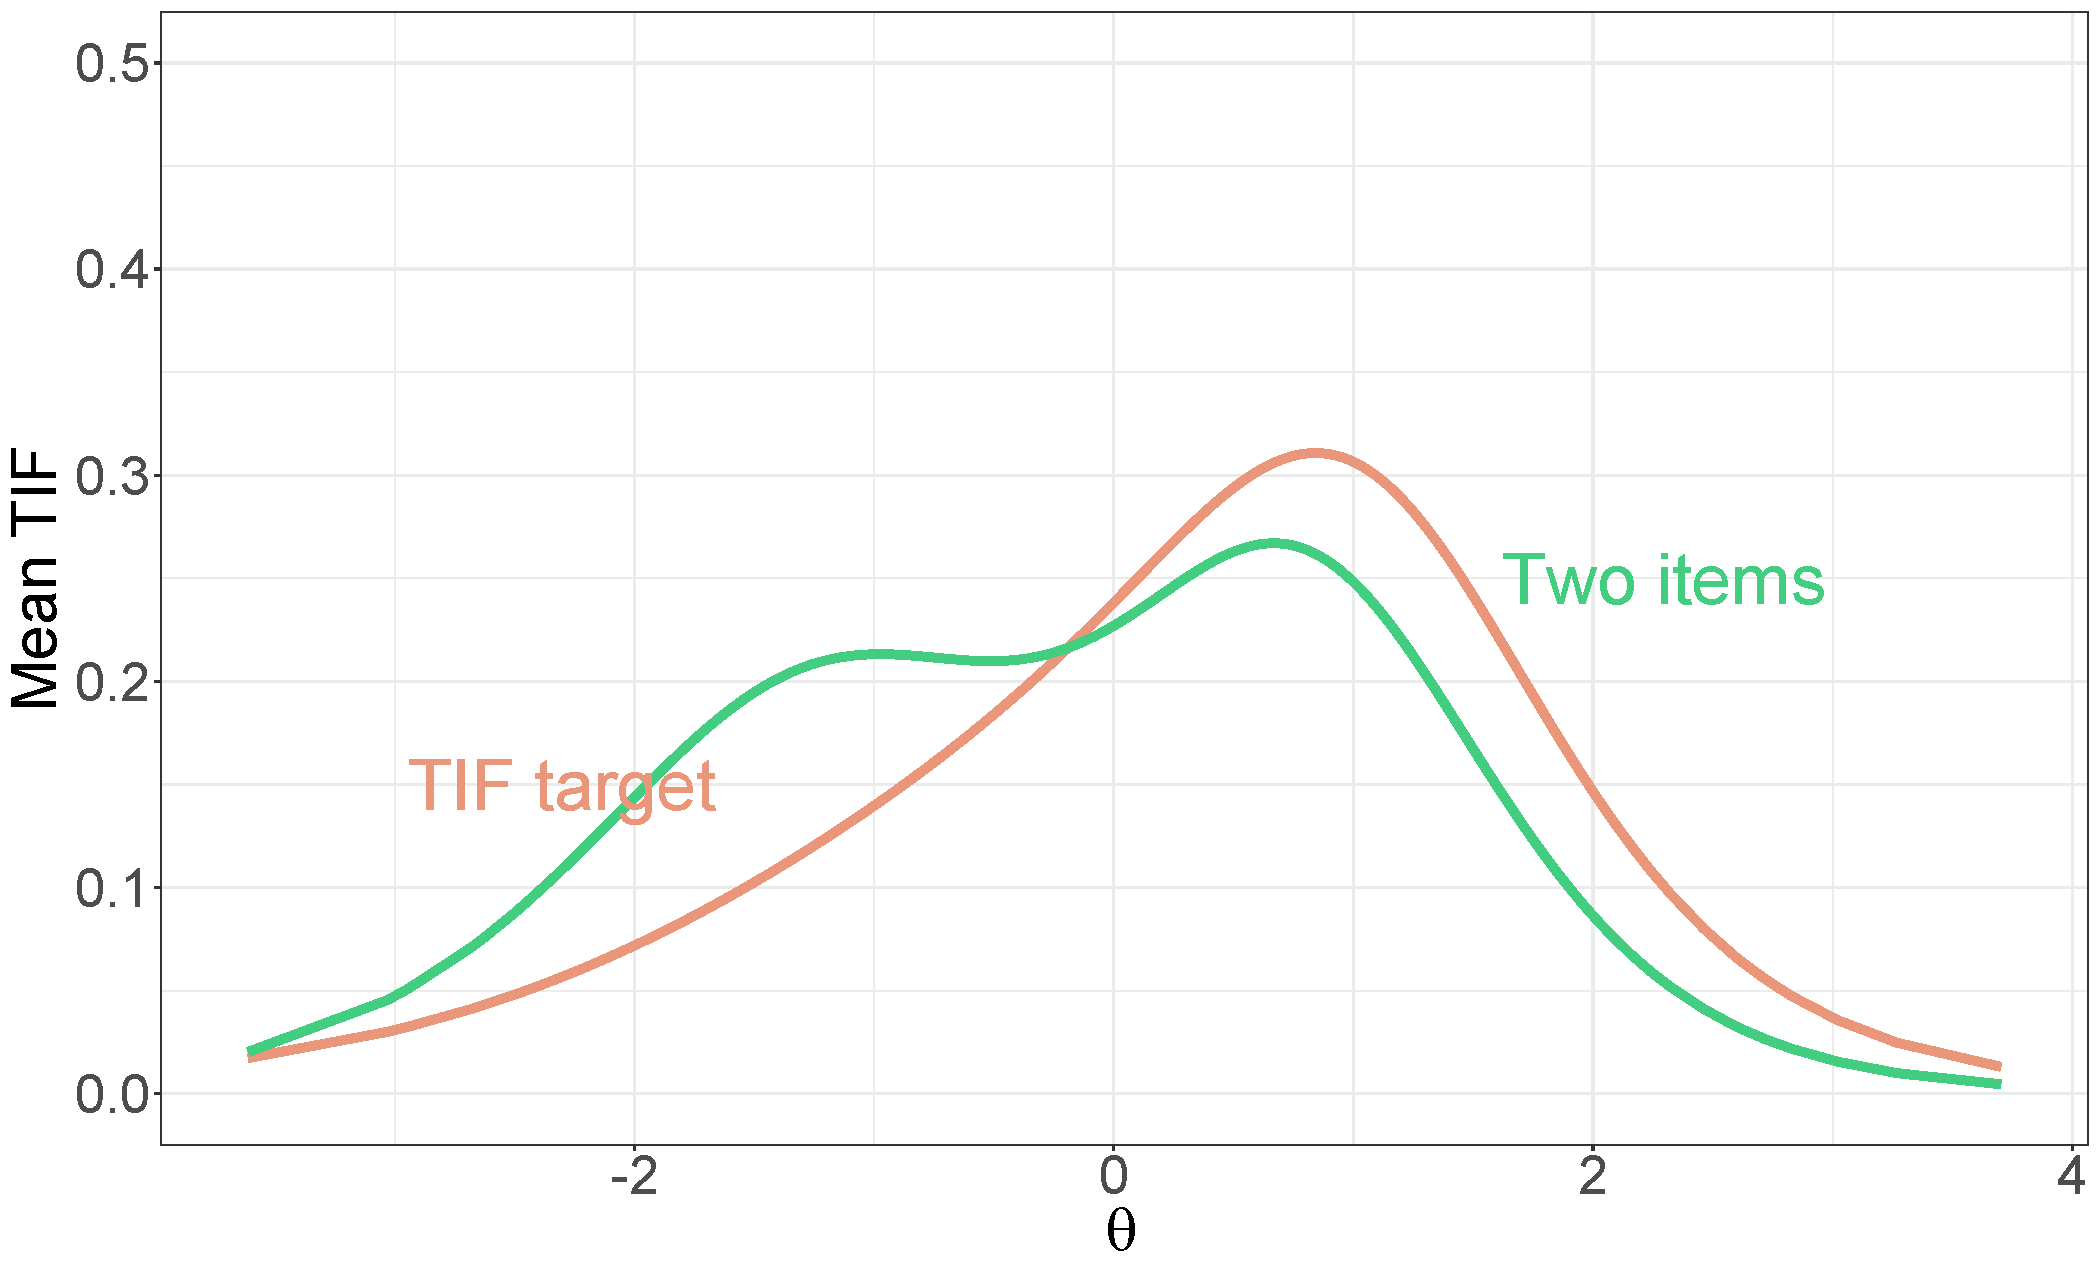
\includegraphics[width=.80\textwidth]{img/TIF-second.pdf}
	
		\onslide<4>
		\centering
	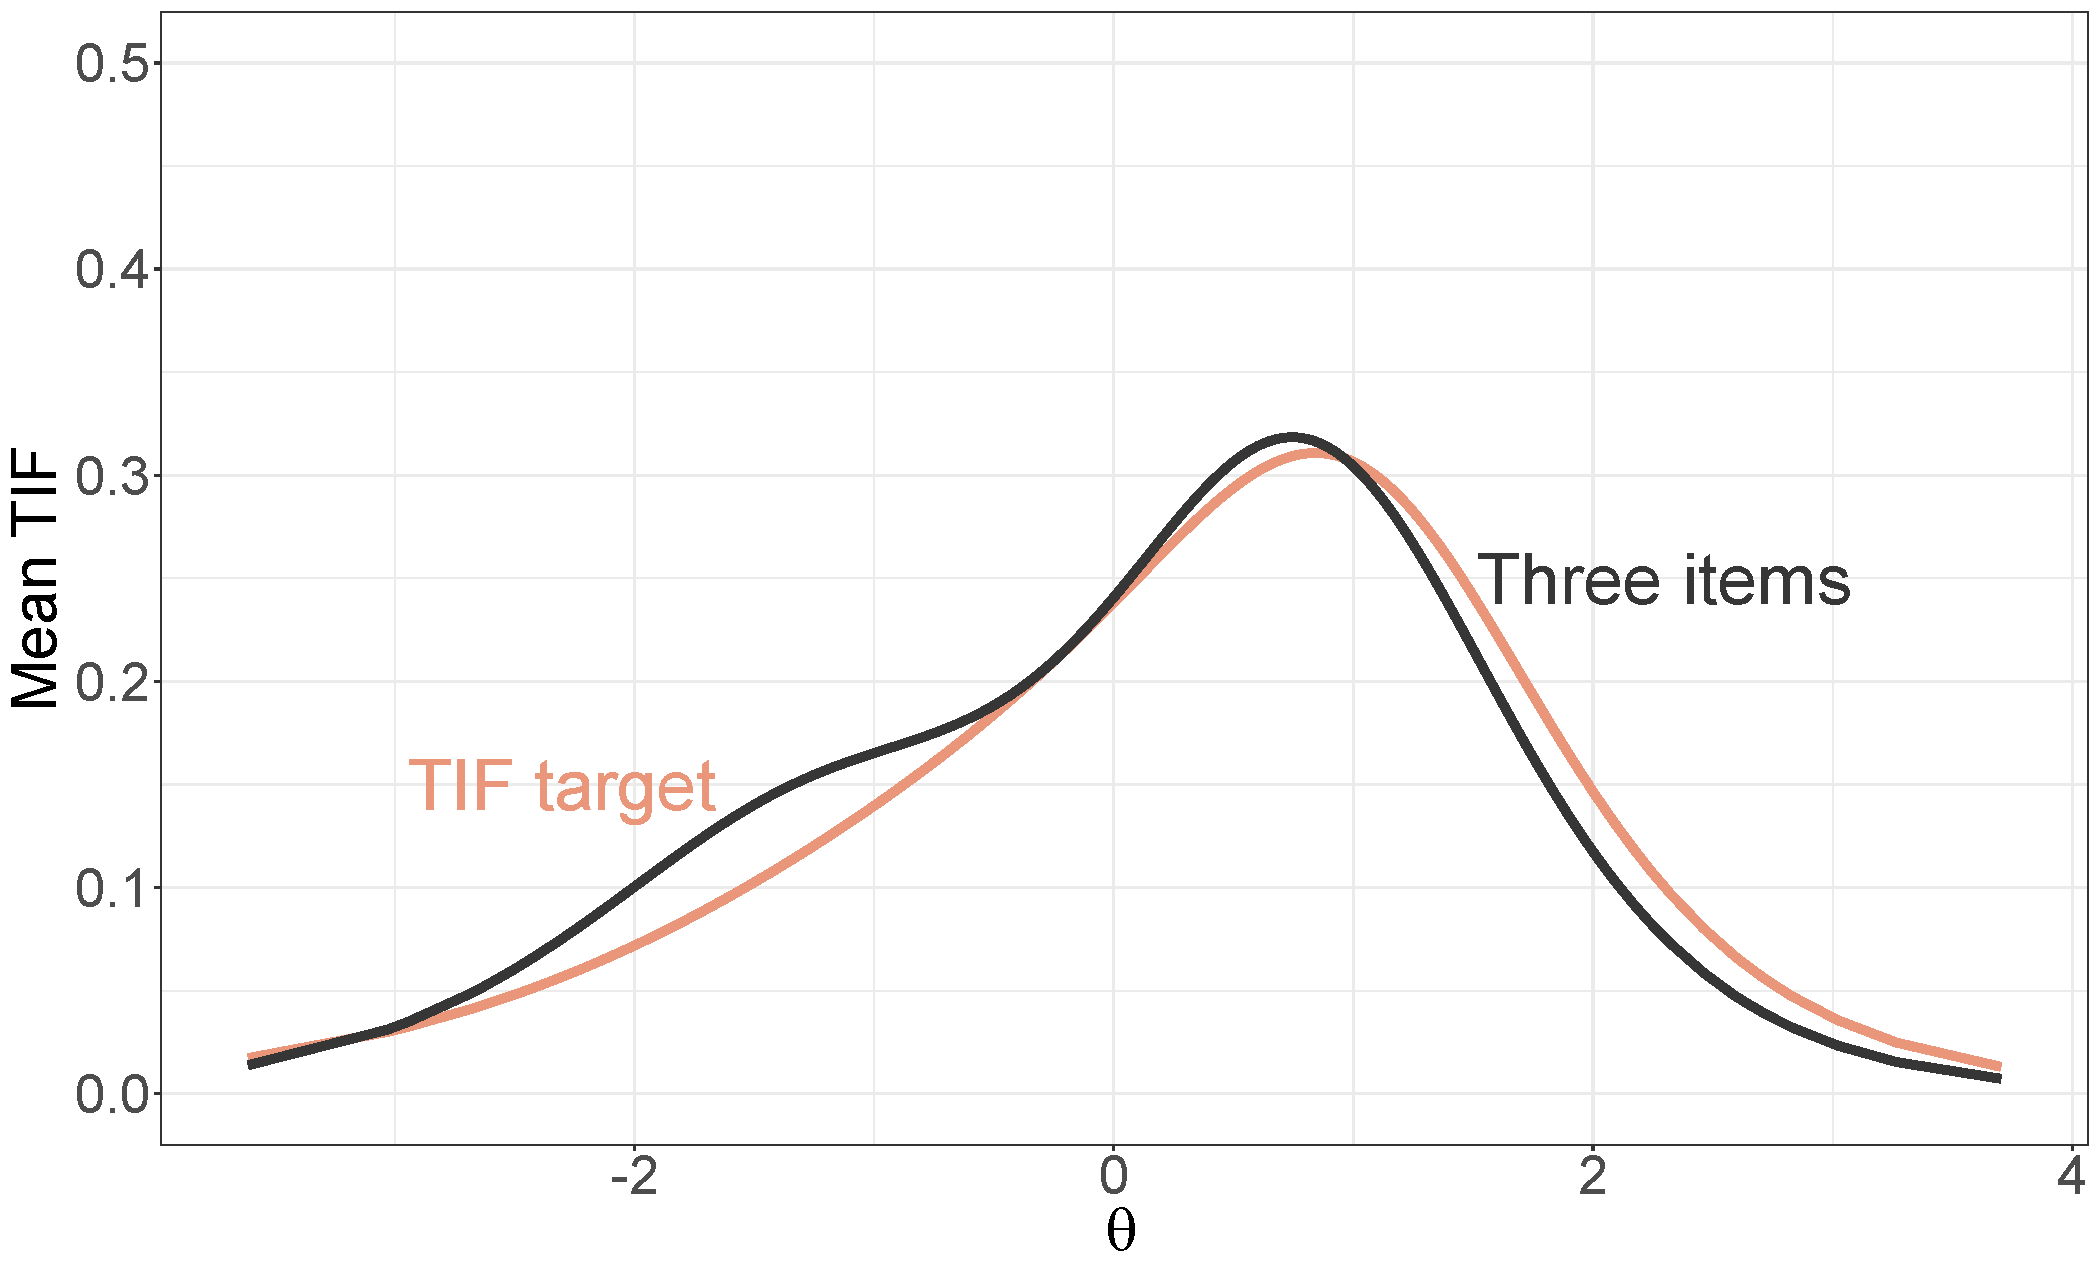
\includegraphics[width=.80\textwidth]{img/TIF-third.pdf}
\end{overprint}
\end{frame}

\section{Latent variables and measurement theory}



\begin{frame}{Measuring fluid intelligence}
	 
	 \small
	 Raven-like measure for the assessment of fluid intelligence in children and adults: From stimulus generation to measure validation under three different approaches
	
	\begin{columns}[T]
		\begin{column}{.50\linewidth}
			\begin{center}
				Classical Test Theory\\
				\small{Factorial solution}
			\end{center}
			\begin{figure}
				\scalebox{.50}{
				\begin{tikzpicture}[node distance=2cm]
					\node (start) [latent] {\Large{g}};
					\node (item1) [item, below of = start, yshift=-1.5cm, xshift=-4.5cm] {Item 32};
					\node (item2) [item, below of = start, yshift=-1.5cm, xshift=-2.5cm] {Item 8};
					\node (itemX) [item, below of = start, yshift=-1.5cm,  xshift=0cm] {$\ldots$};
					\node (item36) [item, below of = start, yshift=-1.5cm, xshift=2.5cm] {Item 21};
					\node (item37) [item, below of = start, yshift=-1.5cm, xshift=4.5cm] {Item 39};
					
					\path [arrow] (start.south) edge node[anchor=west,yshift = -0.4cm, xshift = -2.3cm] {$.48$} (item1.north);
					\path [arrow] (start.south) edge node[anchor=east, yshift = -0.4cm, xshift=-0.6cm] {$.50$} (item2.north);
					\path [arrow] (start.south) edge node[anchor=east, yshift = -0.4cm, xshift=0cm] {$\cdots$} (itemX.north);
					\path [arrow] (start.south) edge node[anchor=east, yshift = - 0.4cm, xshift = 1.4cm] {$.84$} (item36.north);
					\path [arrow] (start.south) edge node[anchor=east, yshift = - 0.4cm, xshift = 2.3cm] {$.84$} (item37.north);
				\end{tikzpicture}
				}
				
			\end{figure}
		\end{column}
		\begin{column}{.50\linewidth}
				\begin{center}
				Rasch modeling\\
				\small{Wright map}
			\end{center}
			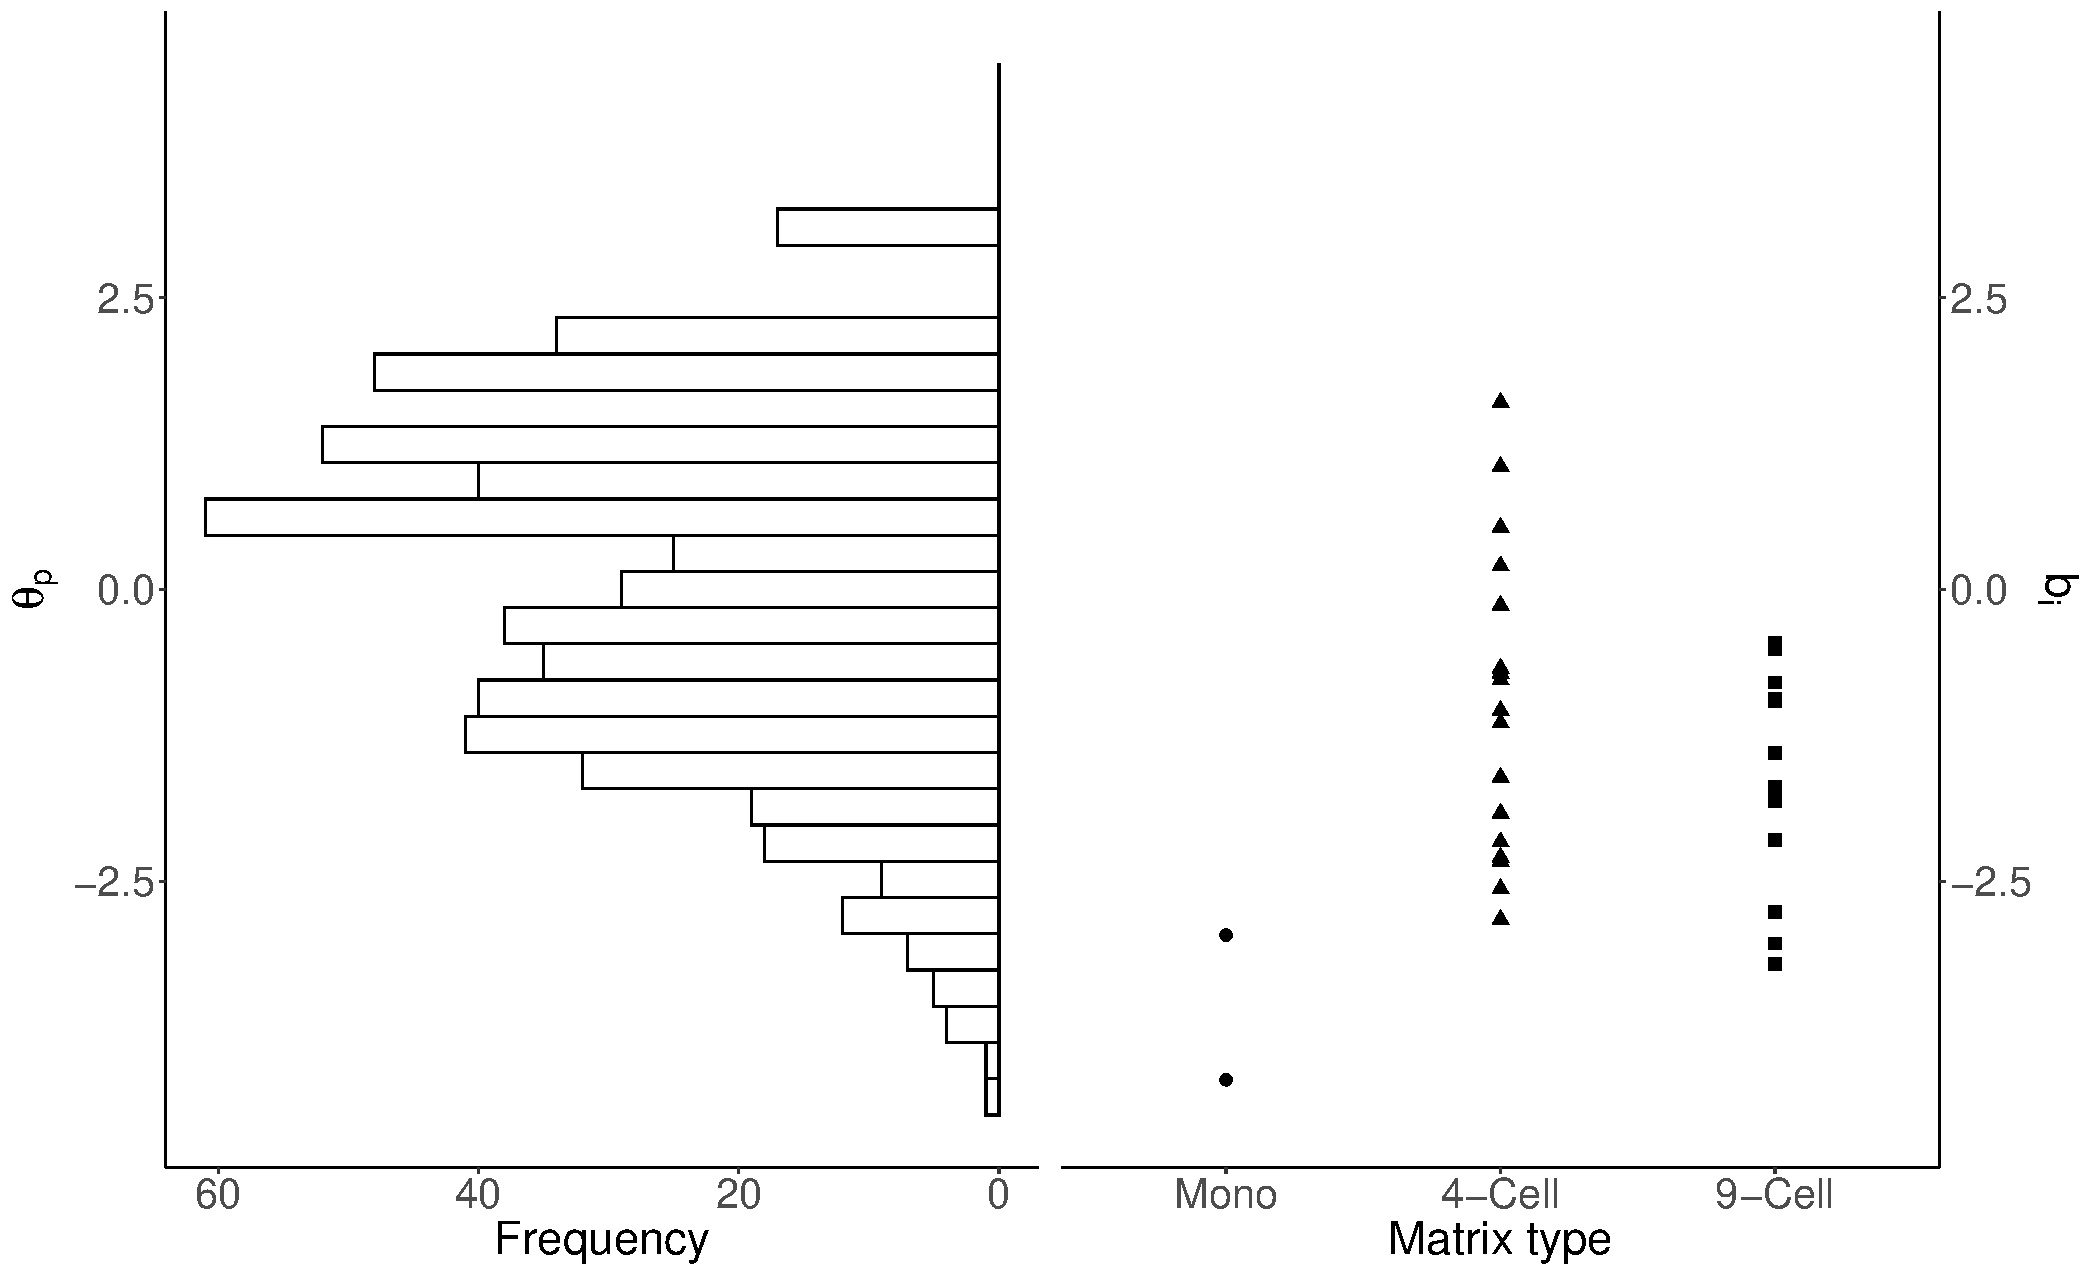
\includegraphics[width=\linewidth]{img/WrightMap.pdf}
		\end{column}
	\end{columns}
	

\end{frame}

\begin{frame}{The meaningfulness of Psychological Measures}
	
	The ratio between the measures of $a$ and $b$ is constant and independent of the measurement unit:
	\[
	\frac{\varphi(a)}{\varphi(b)} = \frac{\varphi'(a)}{\varphi'(b)},
	\]
	
	where $\varphi$ and $\varphi'$ are two different scales of measurement of the same variable.
	
	\begin{block}{Meaningful comparisons}
		
		The comparison between \emph{a} and \emph{b} is meaningful if it is invariant under all the unit transformations. 
		
	\end{block}
\end{frame}


\begin{frame}
\begin{figure}[h]

\scalebox{.80}{
			\begin{tikzpicture}
	\draw[->,thick] (0,0) -- (12,0) node[right] {time (sec)};
	\draw[thick] (0,-.1) node[below] {$0$} --(0,.1);
	\draw[thick] (3.33,-.1) node[below] {$15$} --(3.33,.1);
	\draw[thick] (5.55,-.1) node[below] {$25$} --(5.55,.1);	
	\draw[thick] (6.66,-.1) node[below] {$30$} --(6.66,.1);	
	\draw[thick] (10,-.1) node[below] {$45$} --(10,.1);	
%	\draw[thick] (10,-.1) node[below] {$60$} --(10,.1);	
	\node at (1.7,.5) {$4$};
	\node at (4.75,.5) {$3$};
	\node at (6,.5) {$2$};
	\node at (8.25,.5) {$1$};
	\node at (10.5,.5) {$0$};
%	\node at (10.5,.5) {$0$};
	\node at (-1,0) {\Large\color{unipd}$\varphi$};
\end{tikzpicture}

}

\end{figure}

\begin{figure}
	\scalebox{.80}{
		\begin{tikzpicture}
		\draw[->, thick] (0,0) -- (12,0) node[right] {time (sec)};
	\draw[thick] (0,-.1) node[below] {$0$} --(0,.1);
\draw[thick] (4.44,-.1) node[below] {$20$} --(4.44,.1);
\draw[thick] (6.66,-.1) node[below] {$30$} --(6.66,.1);	
\draw[thick] (7.77,-.1) node[below] {$35$} --(7.77,.1);	
\draw[thick] (11.11,-.1) node[below] {$50$} --(11.11,.1);	
		\node at (2.22,.5) {$4$};
		\node at (5.55,.5) {$3$};
		\node at (7,.5) {$2$};
		\node at (9.25,.5) {$1$};
		\node at (11.5,.5) {$0$};
		\node at (-1,0) {\Large\color{royalblue3}$\varphi'$};
	\end{tikzpicture}
	}

\end{figure}


\onslide<2->
\begin{table}
	\begin{tabular}{cccc ccc cc}
		\hline


Item	&	$t_A$	&	$t_B$	&	&	$\varphi_A$	&	$\varphi_B$	&	&	$\varphi_A'$	&	$\phi_B'$	\\\hline
1	&	14	&	14	&	&	4	&	4	&	&	4	&	4	\\
2	&	26	&	19	&	&	2	&	3	&	&	3	&	4	\\
3	&	31	&	33	&	&	1	&	1	&	&	3	&	2	\\
4	&	46	&	18	&	&	0	&	3	&	&	1	&	4	\\
5	&	17	&	46	&	&	4	&	0	&	&	3	&	1	\\
\hline
Sum scores: & & & & 11 & 11 & & 14 & 15 \\

\hline

	\end{tabular}
\end{table}		
\visible<3> {
	\begin{tikzpicture}[overlay]
		\draw[unipd,ultra thick,rounded corners] (6.7,0) rectangle (8.5,4);
	\end{tikzpicture}
}   

\visible<4> {
	\begin{tikzpicture}[overlay]
		\draw[royalblue3,ultra thick,rounded corners] (9,0.5) rectangle (11,4.5);
	\end{tikzpicture}
}   

\end{frame}


\section{Teaching Activity}

\begin{frame}
	
\begin{block}{In theory (but with practical applications)}
	
	Psychometrics 
	
	Statistics and data analysis in Social Sciences
	
	Measurement Theory and Measurement models in Psychology 
	
	Rasch modeling and Item Response Theory
	
\end{block}

\begin{block}{In practice}
	
	\texttt{R} for beginne\texttt{R}s
	
	RMarkdown in an Open Science perspective
	
	Developing  web applications with \texttt{shiny}
	
	Implementing experiments in Inquisit
	
\end{block}
	
\end{frame}


\appendix

\begin{frame}[plain]
	\begin{center}
		\Large
		Thank you! 
		
		\begin{figure}
			\centering
			
\includegraphics[width=.4\linewidth]{img/OME.png}
		\end{figure}
		
	\end{center}
\end{frame}

\end{document}
